\documentclass[10pt]{report}
\usepackage{ctex}
\usepackage[utf8]{inputenc}
\usepackage{amsmath}
\usepackage{amssymb}
\usepackage{xcolor}
\usepackage{graphicx}
\usepackage[margin=0.1cm]{geometry} % 设置页边距为 0.5cm，尽可能扩大可用区域
\usepackage{setspace}
\renewcommand{\baselinestretch}{1} % 设置行间距为单倍行距
\usepackage{float}
\usepackage{wrapfig}
\usepackage[utf8]{inputenc}
\usepackage[T1]{fontenc}
\usepackage{ctex}
\usepackage{amsmath}
\usepackage{amssymb}
\usepackage{xcolor}
\usepackage{graphicx}
\usepackage{float}
\usepackage{lmodern}
\usepackage{mathrsfs}
\usepackage{lipsum}
\usepackage{array} 
\usepackage{amsmath}    % 数学公式
\usepackage{booktabs}   % 专业表格
\usepackage{multirow}   % 多行表格
\usepackage{graphicx}   % 插入图片
\usepackage{siunitx}    % 国际单位
\usepackage{enumitem}   % 列表控制
\usepackage{graphicx}
\usepackage{subcaption} % 支持子图
\usepackage{tikz}
\usepackage{braket}
\usepackage{adjustbox}
\usepackage{footmisc}
\usepackage{array}
\usepackage{multirow}
\usepackage[table]{xcolor}
\usepackage{amsmath}
\usepackage{tcolorbox}
\usepackage{caption}
\usepackage{tabularx}
\captionsetup[figure]{labelformat=empty} % 设置图标题的标签格式为空，即不显示“图 X”
\usepackage{graphicx}
\tcbuselibrary{listings,breakable}
\usepackage{xcolor}
\setlength{\parindent}{0pt}
\captionsetup[figure]{skip=0pt}
\usepackage{array}
\title{PN结}
\author{张世航}
\begin{document}
	\maketitle
	\section{$U_F-I_F$曲线}
	\subsection{$T=298.15K$}
	{
	\resizebox{\textwidth}{!}{ % 宽度撑满文本宽度，高度自动调整
		\begin{tabular}{|c|*{23}{c|}}
			\hline
			序号 &1 & 2 & 3 & 4 & 5 & 6 & 7 & 8 & 9 & 10 & 11 &12 &13&14&15&16&17&18&19&20&21&22&23  \\
			\hline
			$U_F$(V) &0.350 & 0.360 & 0.370 & 0.380 & 0.390 & 0.400 & 0.410 & 0.420 & 0.430 & 0.440 & 0.450 & 0.460 & 0.470 & 0.480 & 0.490 & 0.500 & 0.510 & 0.520 & 0.530 & 0.540 & 0.550 & 0.560 & 0.570  \\
			\hline
			$I_F$($\mu$A) &0.017 & 0.026 & 0.041 & 0.062 & 0.092 & 0.138 & 0.205 & 0.299 & 0.442 & 0.648 & 0.960 & 1.400 & 2.060 & 3.060 & 4.490 & 6.660 & 9.970 & 14.400 & 21.200 & 31.500 & 46.100 & 67.200 & 99.000 \\
			\hline
		\end{tabular}
	}
	\begin{figure}[H]
		\centering
		\begin{subfigure}{0.48\textwidth} % 第一个子图，宽度占文本的48%
			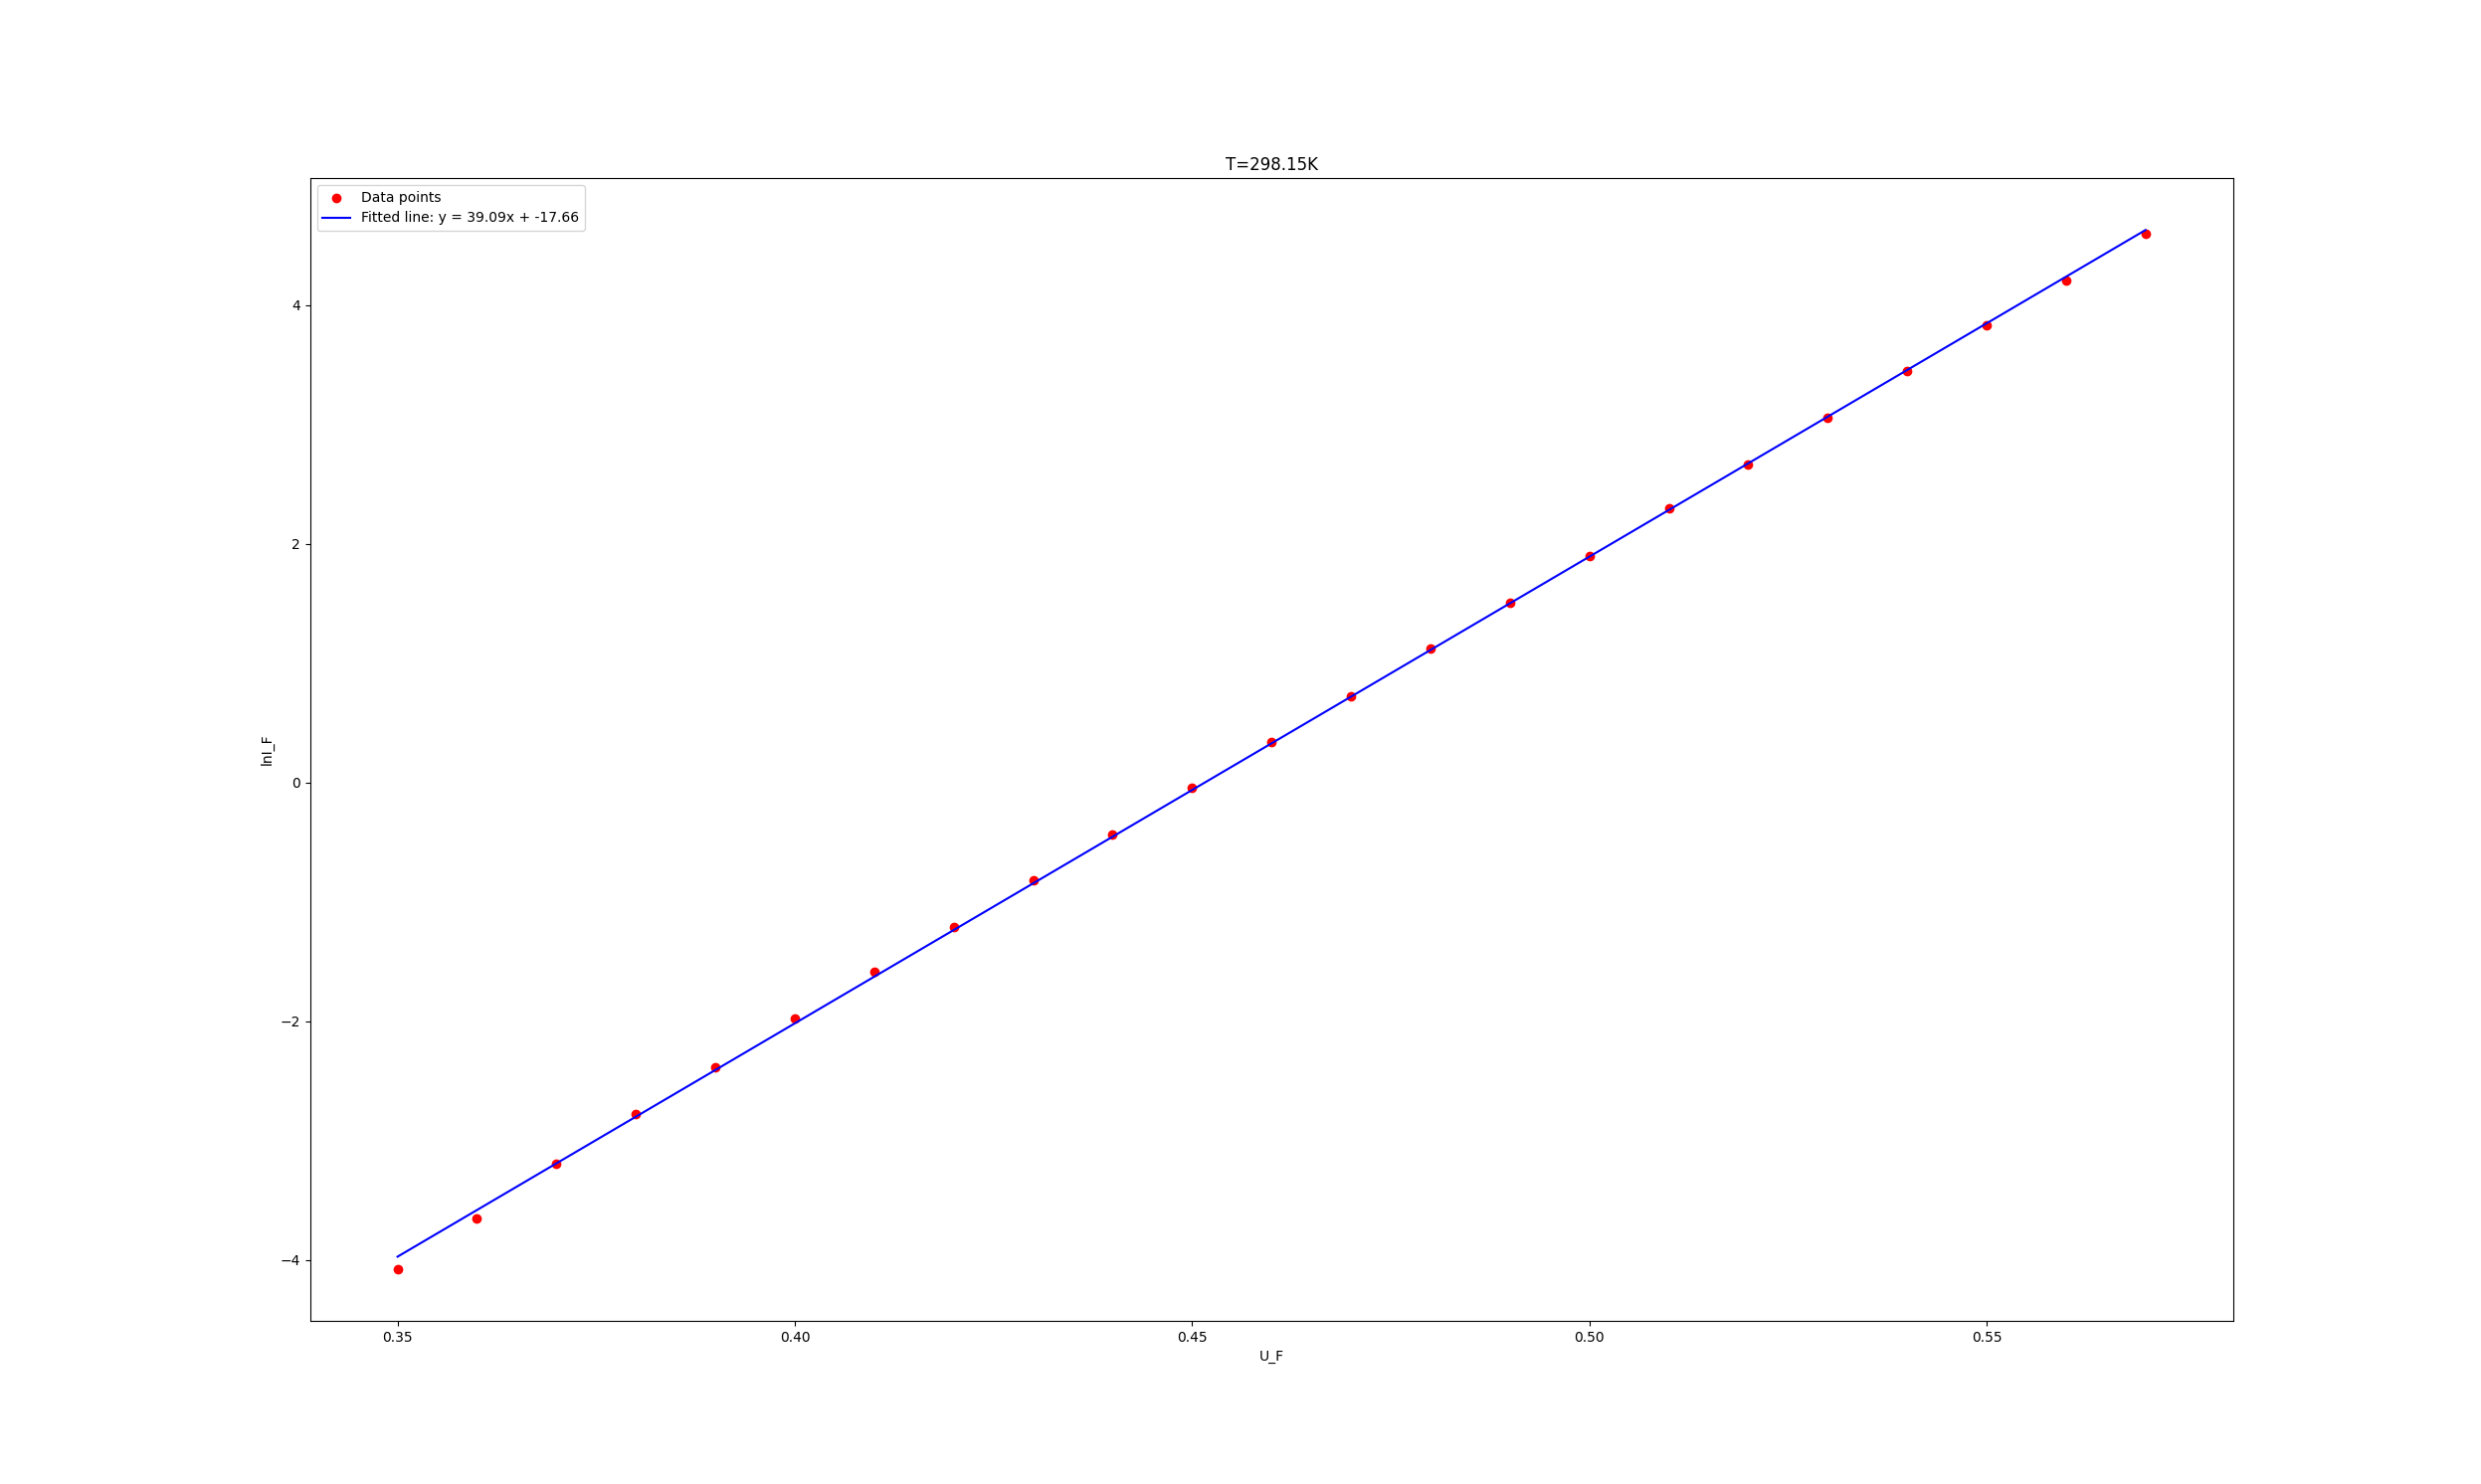
\includegraphics[width=\linewidth]{1.1.1.png}
			\caption{$lnI_F=39.09U_F-17.66$}
			\label{fig:sub1}
		\end{subfigure}
		\hfill % 填充水平间距
		\begin{subfigure}{0.48\textwidth} % 第二个子图
			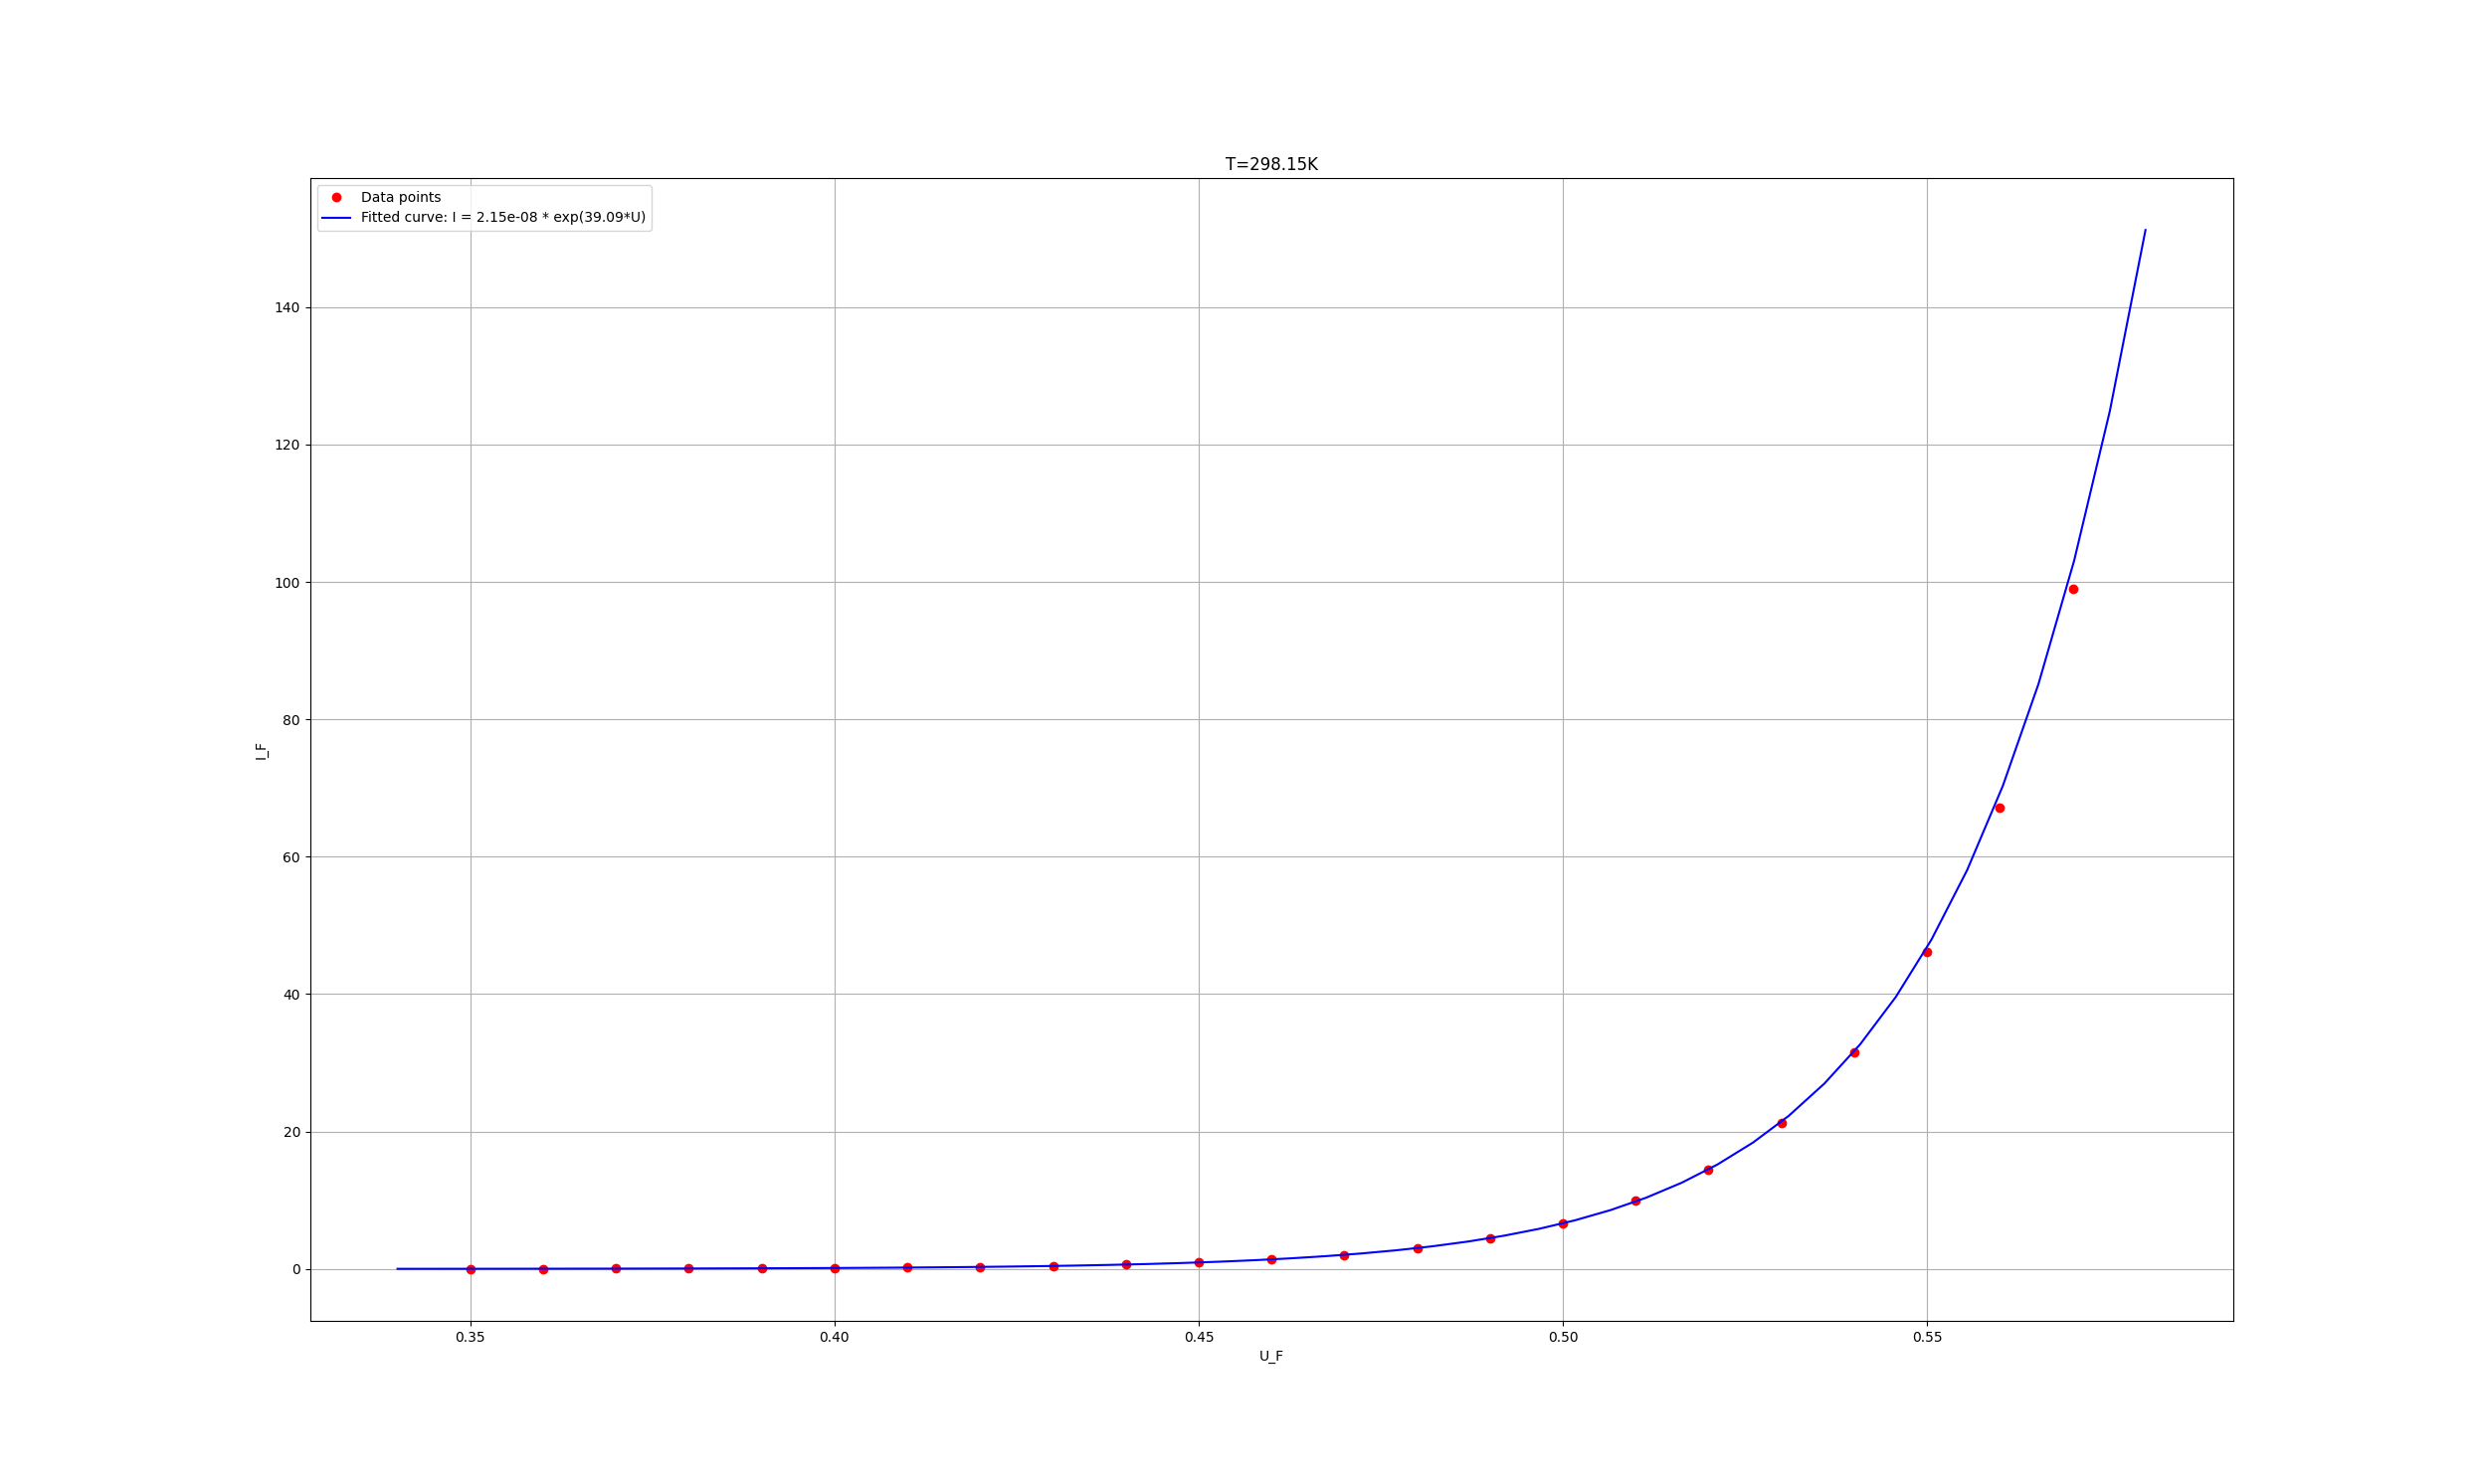
\includegraphics[width=\linewidth]{1.1.2.png}
			\caption{$I_F=2.15\times 10^{-8}e^{39.09U_F}$}
			\label{fig:sub2}
		\end{subfigure}
		\caption{$T=298.15K$}
		\label{fig1:combined}
	\end{figure}

    对于\[I_F = I_s exp(\frac{qV_F}{kT})\]
    我们可以得到 \[I_s = 2.15\times 10^{-8}\mu A,\frac{q}{kT} = 39.09V^{-1}\]
    我们可以计算出 \[k = \frac{q}{T\times39.09V^{-1}} = \frac{1.6\times10^{-19}C}{298.15K\times39.09V^{-1}}=1.3722838653\times10^{-23}J/K\]
    对于玻尔兹曼常数的公认值为\[k = 1.380649\times10^{-23} J/K\]
    我们的误差为\[\frac{|1.380649\times10^{-23} J/K-1.3722838653\times10^{-23}J/K|}{1.380649\times10^{-23} J/K}\times100\%=0.6059\%\]
}
	\subsection{$T=313.15K$}
	{
	\resizebox{\textwidth}{!}{ % 宽度撑满文本宽度，高度自动调整
		\begin{tabular}{|c|*{23}{c|}}
			\hline
			序号 &1 & 2 & 3 & 4 & 5 & 6 & 7 & 8 & 9 & 10 & 11 &12 &13&14&15&16&17&18&19&20&21&22&23  \\
			\hline
			$U_F$(V) &0.350 & 0.360 & 0.370 & 0.380 & 0.390 & 0.400 & 0.410 & 0.420 & 0.430 & 0.440 & 0.450 & 0.460 & 0.470 & 0.480 & 0.490 & 0.500 & 0.510 & 0.520 & 0.530 & 0.540 & 0.550 & 0.560 & 0.570  \\
			\hline
			$I_F$($\mu$A) &0.114 & 0.166 & 0.234 & 0.333 & 0.482 & 0.678 & 0.952 & 1.340 & 1.920 & 2.710 & 4.370 & 6.720 & 8.200 & 11.800 & 17.800 & 26.200 & 38.700 & 57.300 & 83.300 & 132.000 & 187.000 & 274.000 & 395.000\\
			\hline
		\end{tabular}
	}
	\begin{figure}[H]
		\centering
		\begin{subfigure}{0.48\textwidth} % 第一个子图，宽度占文本的48%
			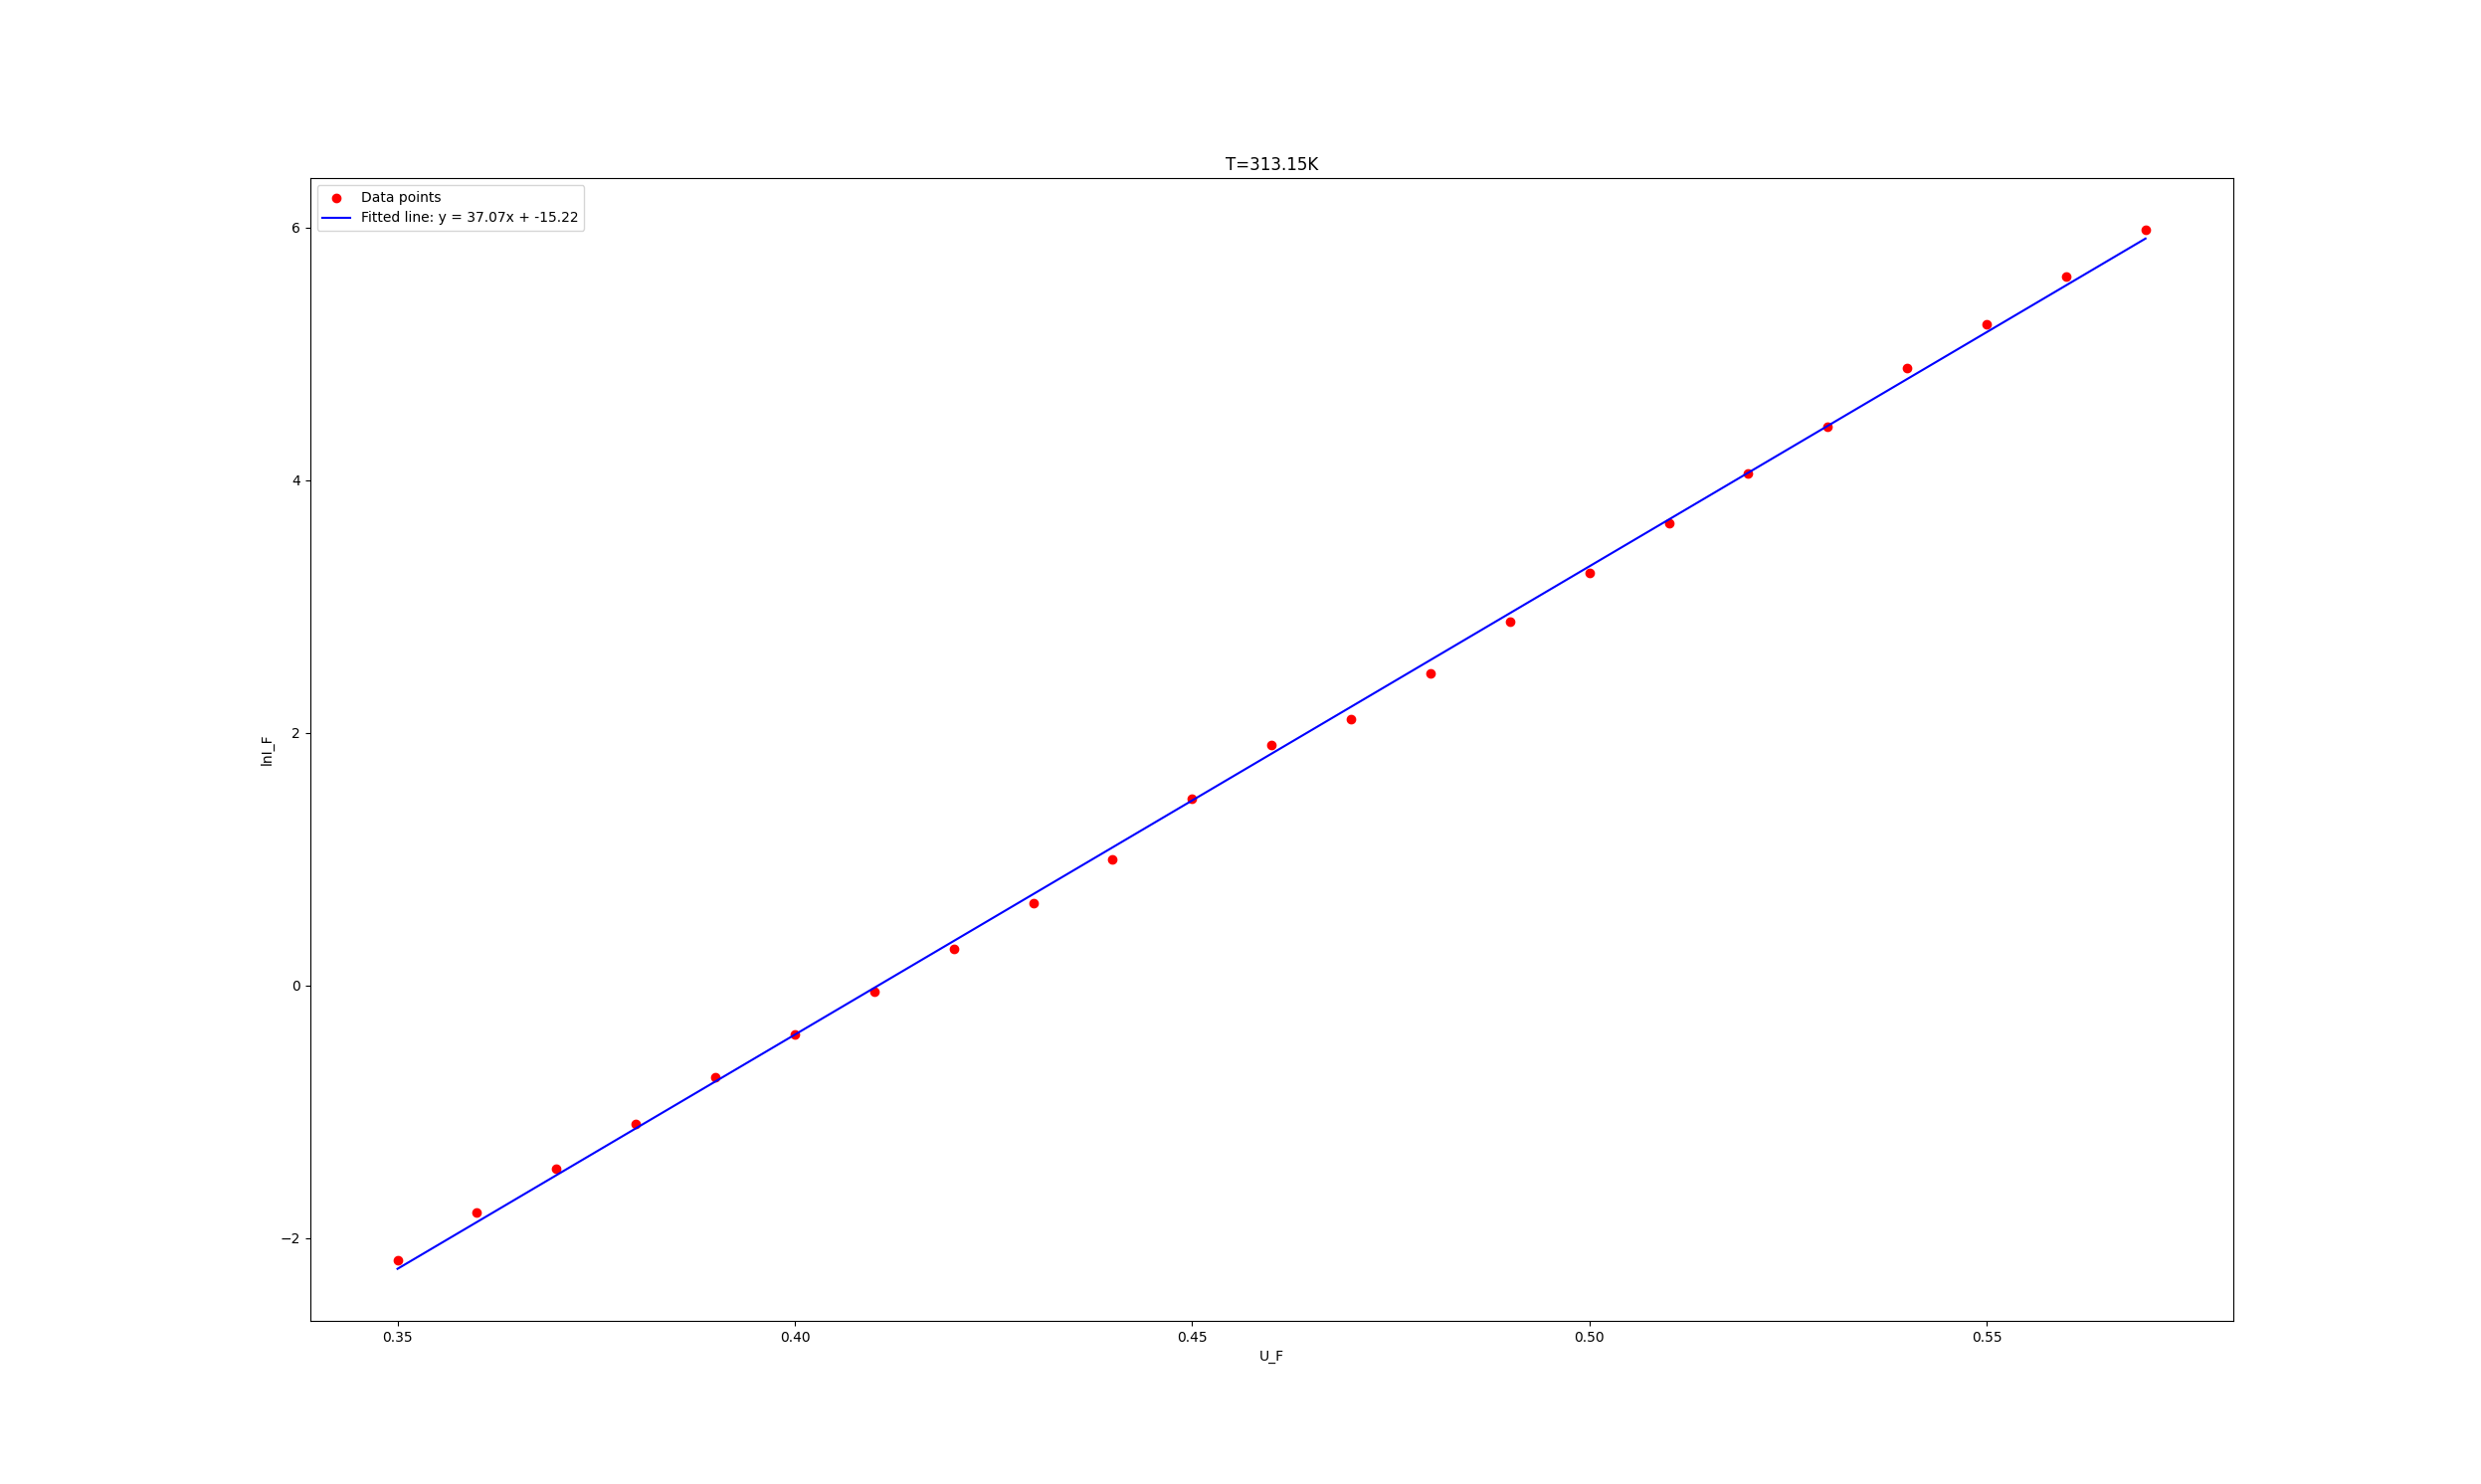
\includegraphics[width=\linewidth]{1.2.1.png}
			\caption{$lnI_F=37.07U_F-15.22$}
			\label{fig:sub3}
		\end{subfigure}
		\hfill % 填充水平间距
		\begin{subfigure}{0.48\textwidth} % 第二个子图
			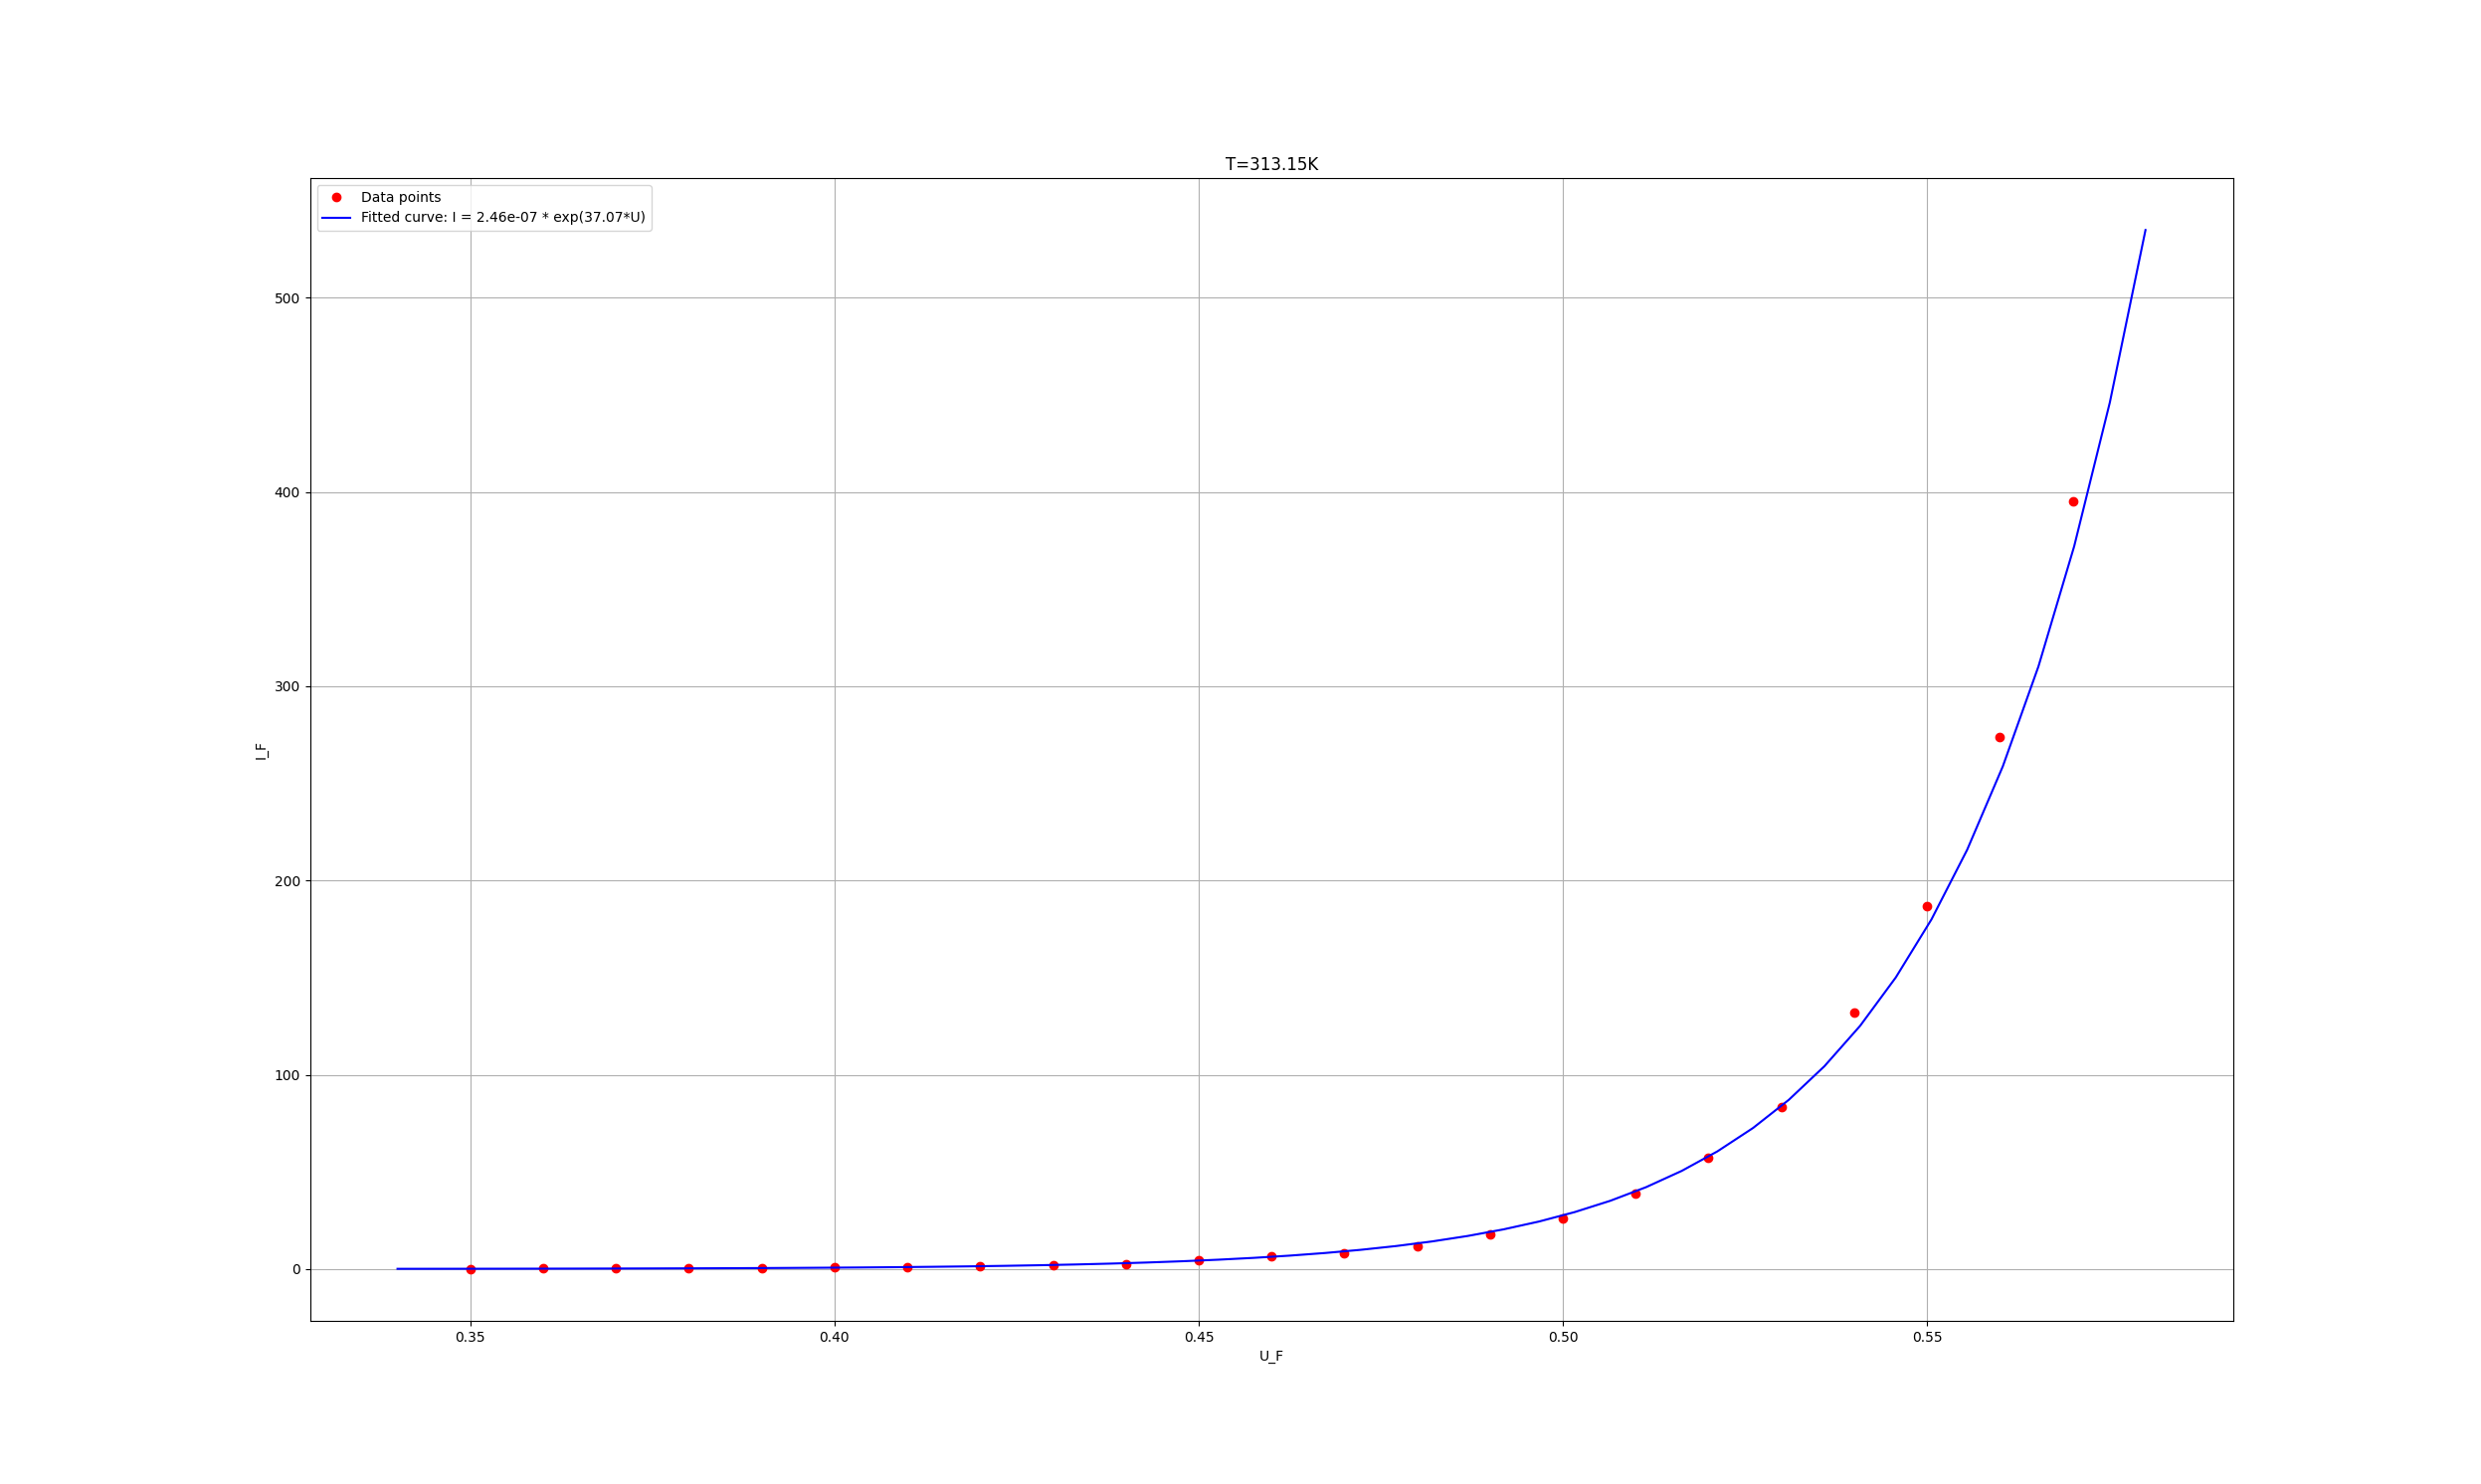
\includegraphics[width=\linewidth]{1.2.2.png}
			\caption{$I_F=2.46\times 10^{-7}e^{37.07U_F}$}
			\label{fig:sub4}
		\end{subfigure}
		\caption{$T=313.15K$}
		\label{fig2:combined}
	\end{figure}
    
	我们可以得到 \[I_s = 2.46\times 10^{-7}\mu A,\frac{q}{kT} =37.07V^{-1}\]
	我们可以计算出 \[k = \frac{q}{T\times37.07V^{-1}} = \frac{1.6\times10^{-19}C}{313.15K\times37.07V^{-1}}=1.378303886\times10^{-23}J/K\]
	对于玻尔兹曼常数的公认值为\[k = 1.380649\times10^{-23} J/K\]
	我们的误差为\[\frac{|1.380649\times10^{-23} J/K-1.378303886\times10^{-23}J/K|}{1.380649\times10^{-23} J/K}\times100\%=0.1698559\%\]
    }
	\subsection{$T=328.15K$}
	{
	\resizebox{\textwidth}{!}{ % 宽度撑满文本宽度，高度自动调整
		\begin{tabular}{|c|*{23}{c|}}
			\hline
			序号 &1 & 2 & 3 & 4 & 5 & 6 & 7 & 8 & 9 & 10 & 11 &12 &13&14&15&16&17&18&19&20&21&22&23  \\
			\hline
			$U_F$(V) &0.350 & 0.360 & 0.370 & 0.380 & 0.390 & 0.400 & 0.410 & 0.420 & 0.430 & 0.440 & 0.450 & 0.460 & 0.470 & 0.480 & 0.490 & 0.500 & 0.510 & 0.520 & 0.530 & 0.540 & 0.550 & 0.560 & 0.564\\
			\hline
			$I_F$($\mu$A) & 0.625 & 0.839 & 1.120 & 1.550 & 2.200 & 2.990 & 4.260 & 6.630 & 10.040 & 14.100 & 19.900 & 28.000 & 39.300 & 56.900 & 81.300 & 114.000 & 162.000 & 233.000 & 331.000 & 470.000 & 669.000 & 923.000 & 1059.000\\
			\hline
		\end{tabular}
	}
	\begin{figure}[H]
		\centering
		\begin{subfigure}{0.48\textwidth} % 第一个子图，宽度占文本的48%
			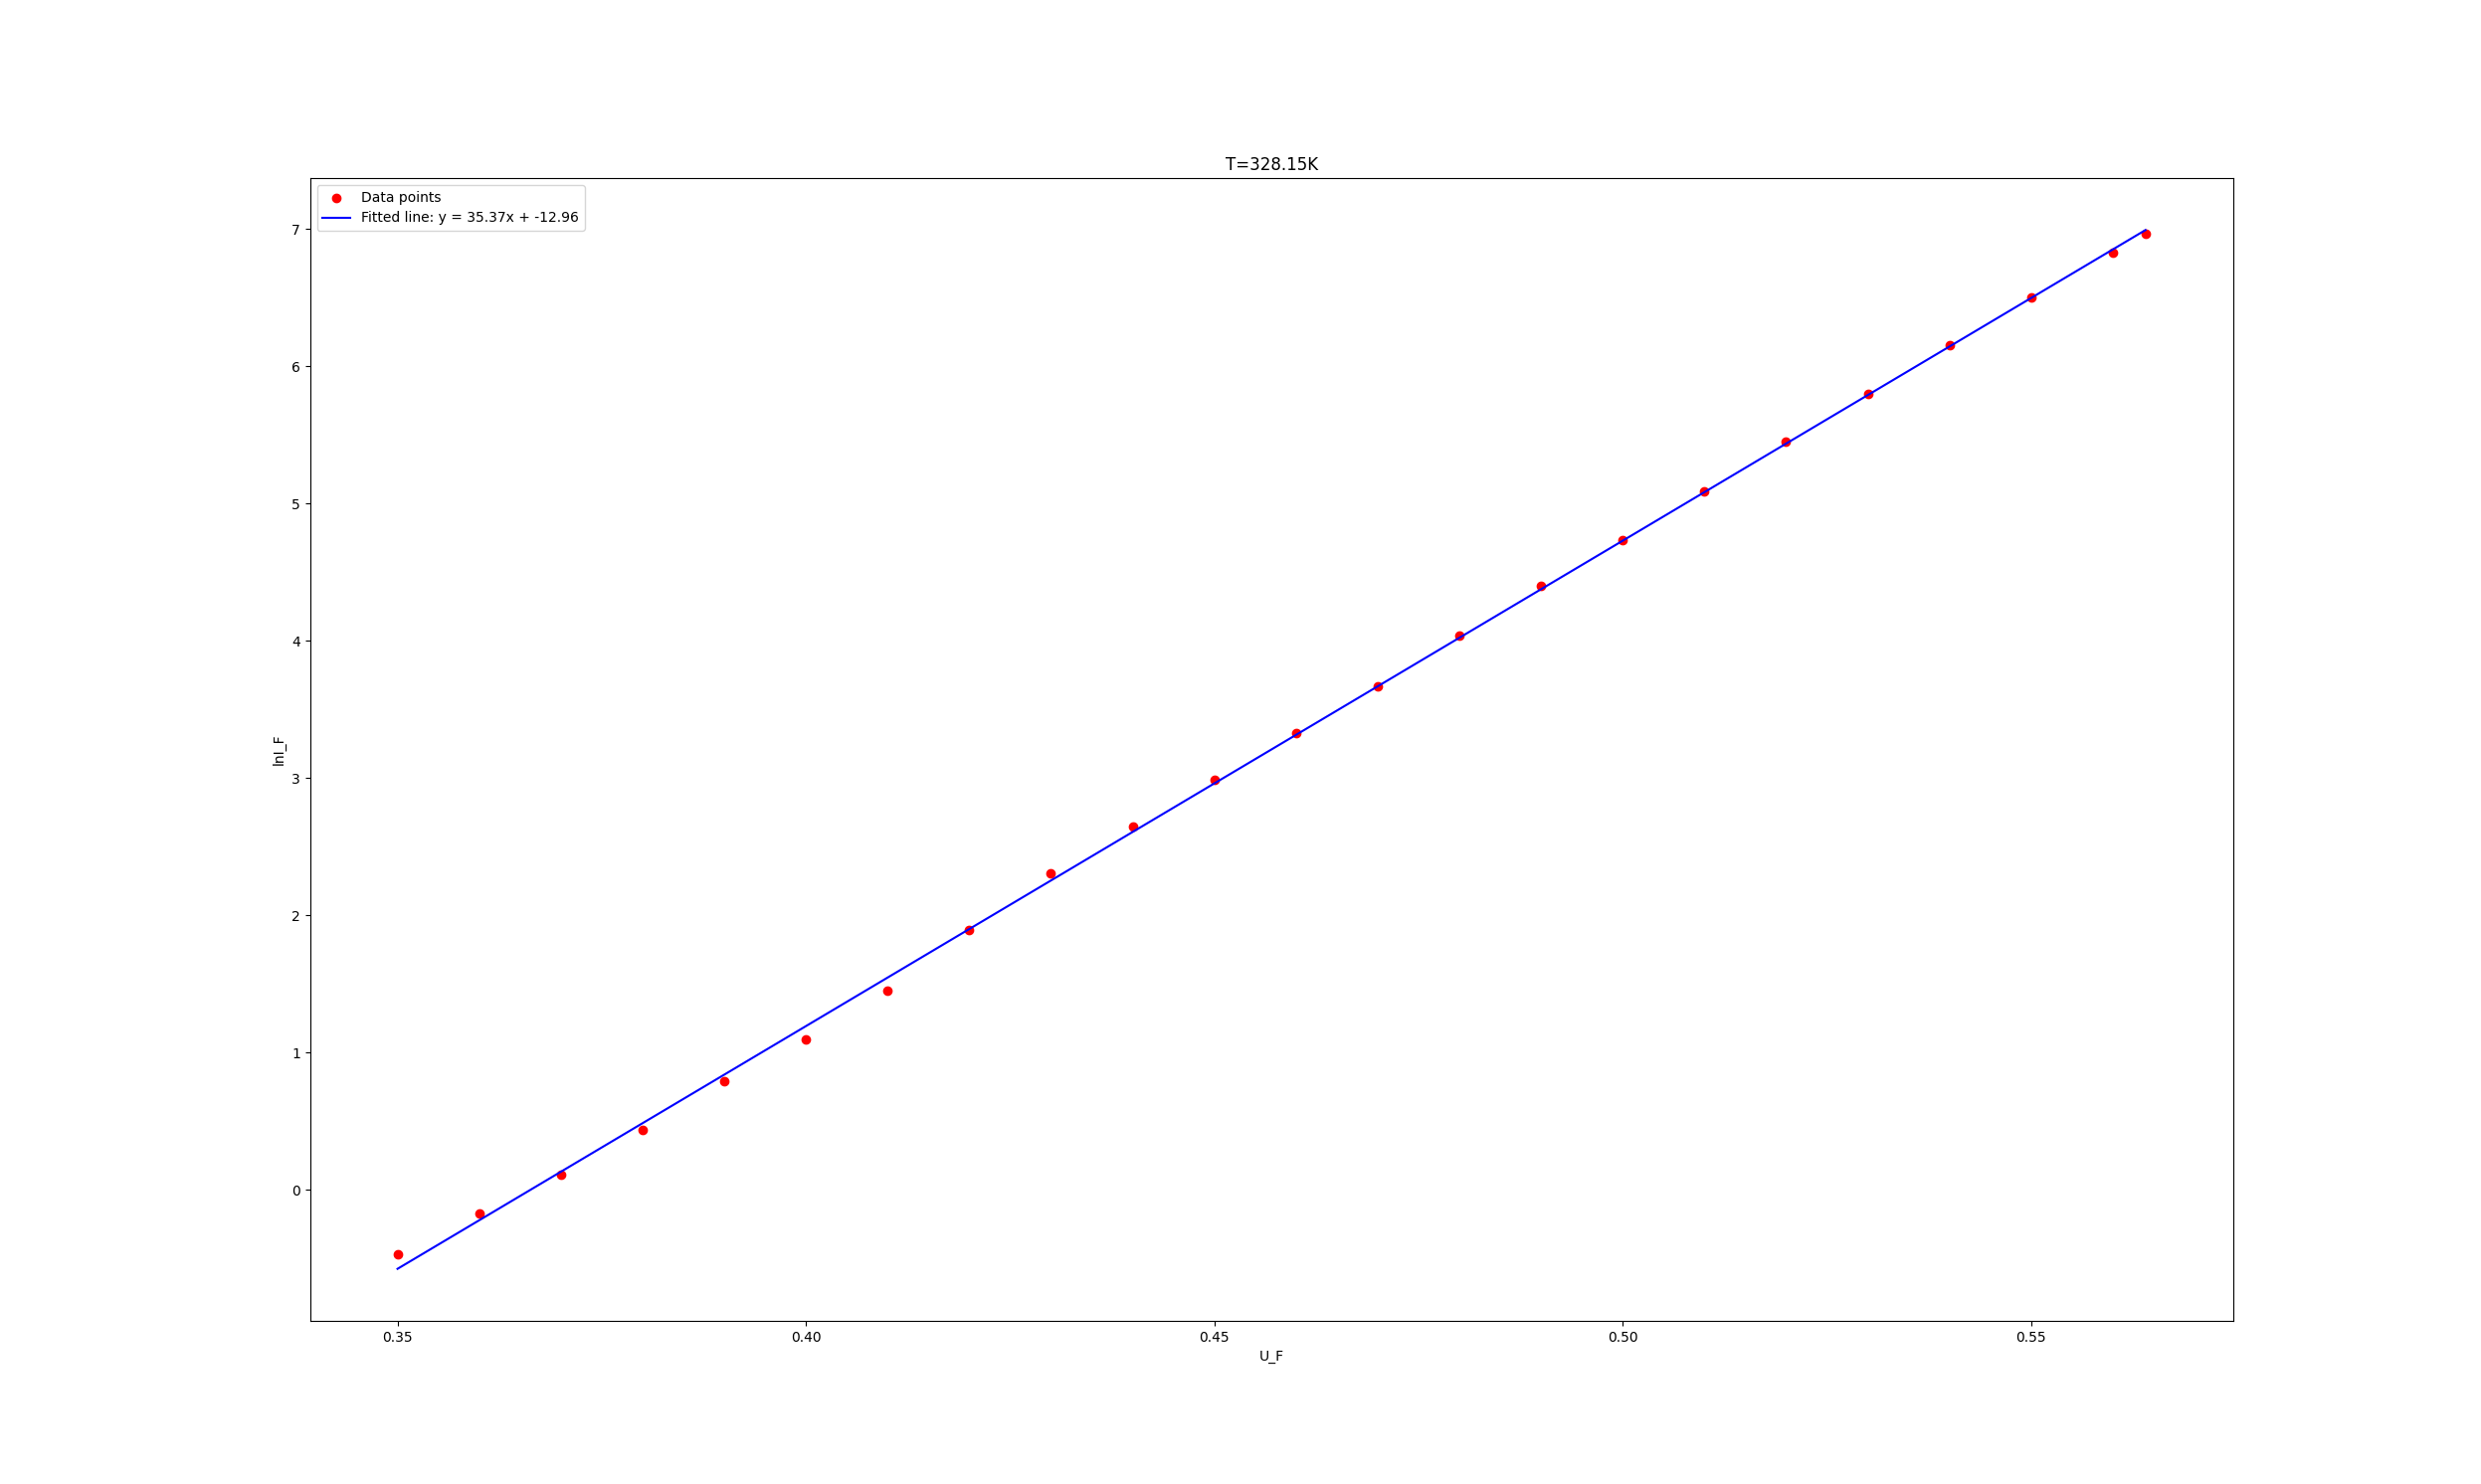
\includegraphics[width=\linewidth]{1.3.1.png}
			\caption{$lnI_F=35.37U_F-12.96$}
			\label{fig:sub5}
		\end{subfigure}
		\hfill % 填充水平间距
		\begin{subfigure}{0.48\textwidth} % 第二个子图
			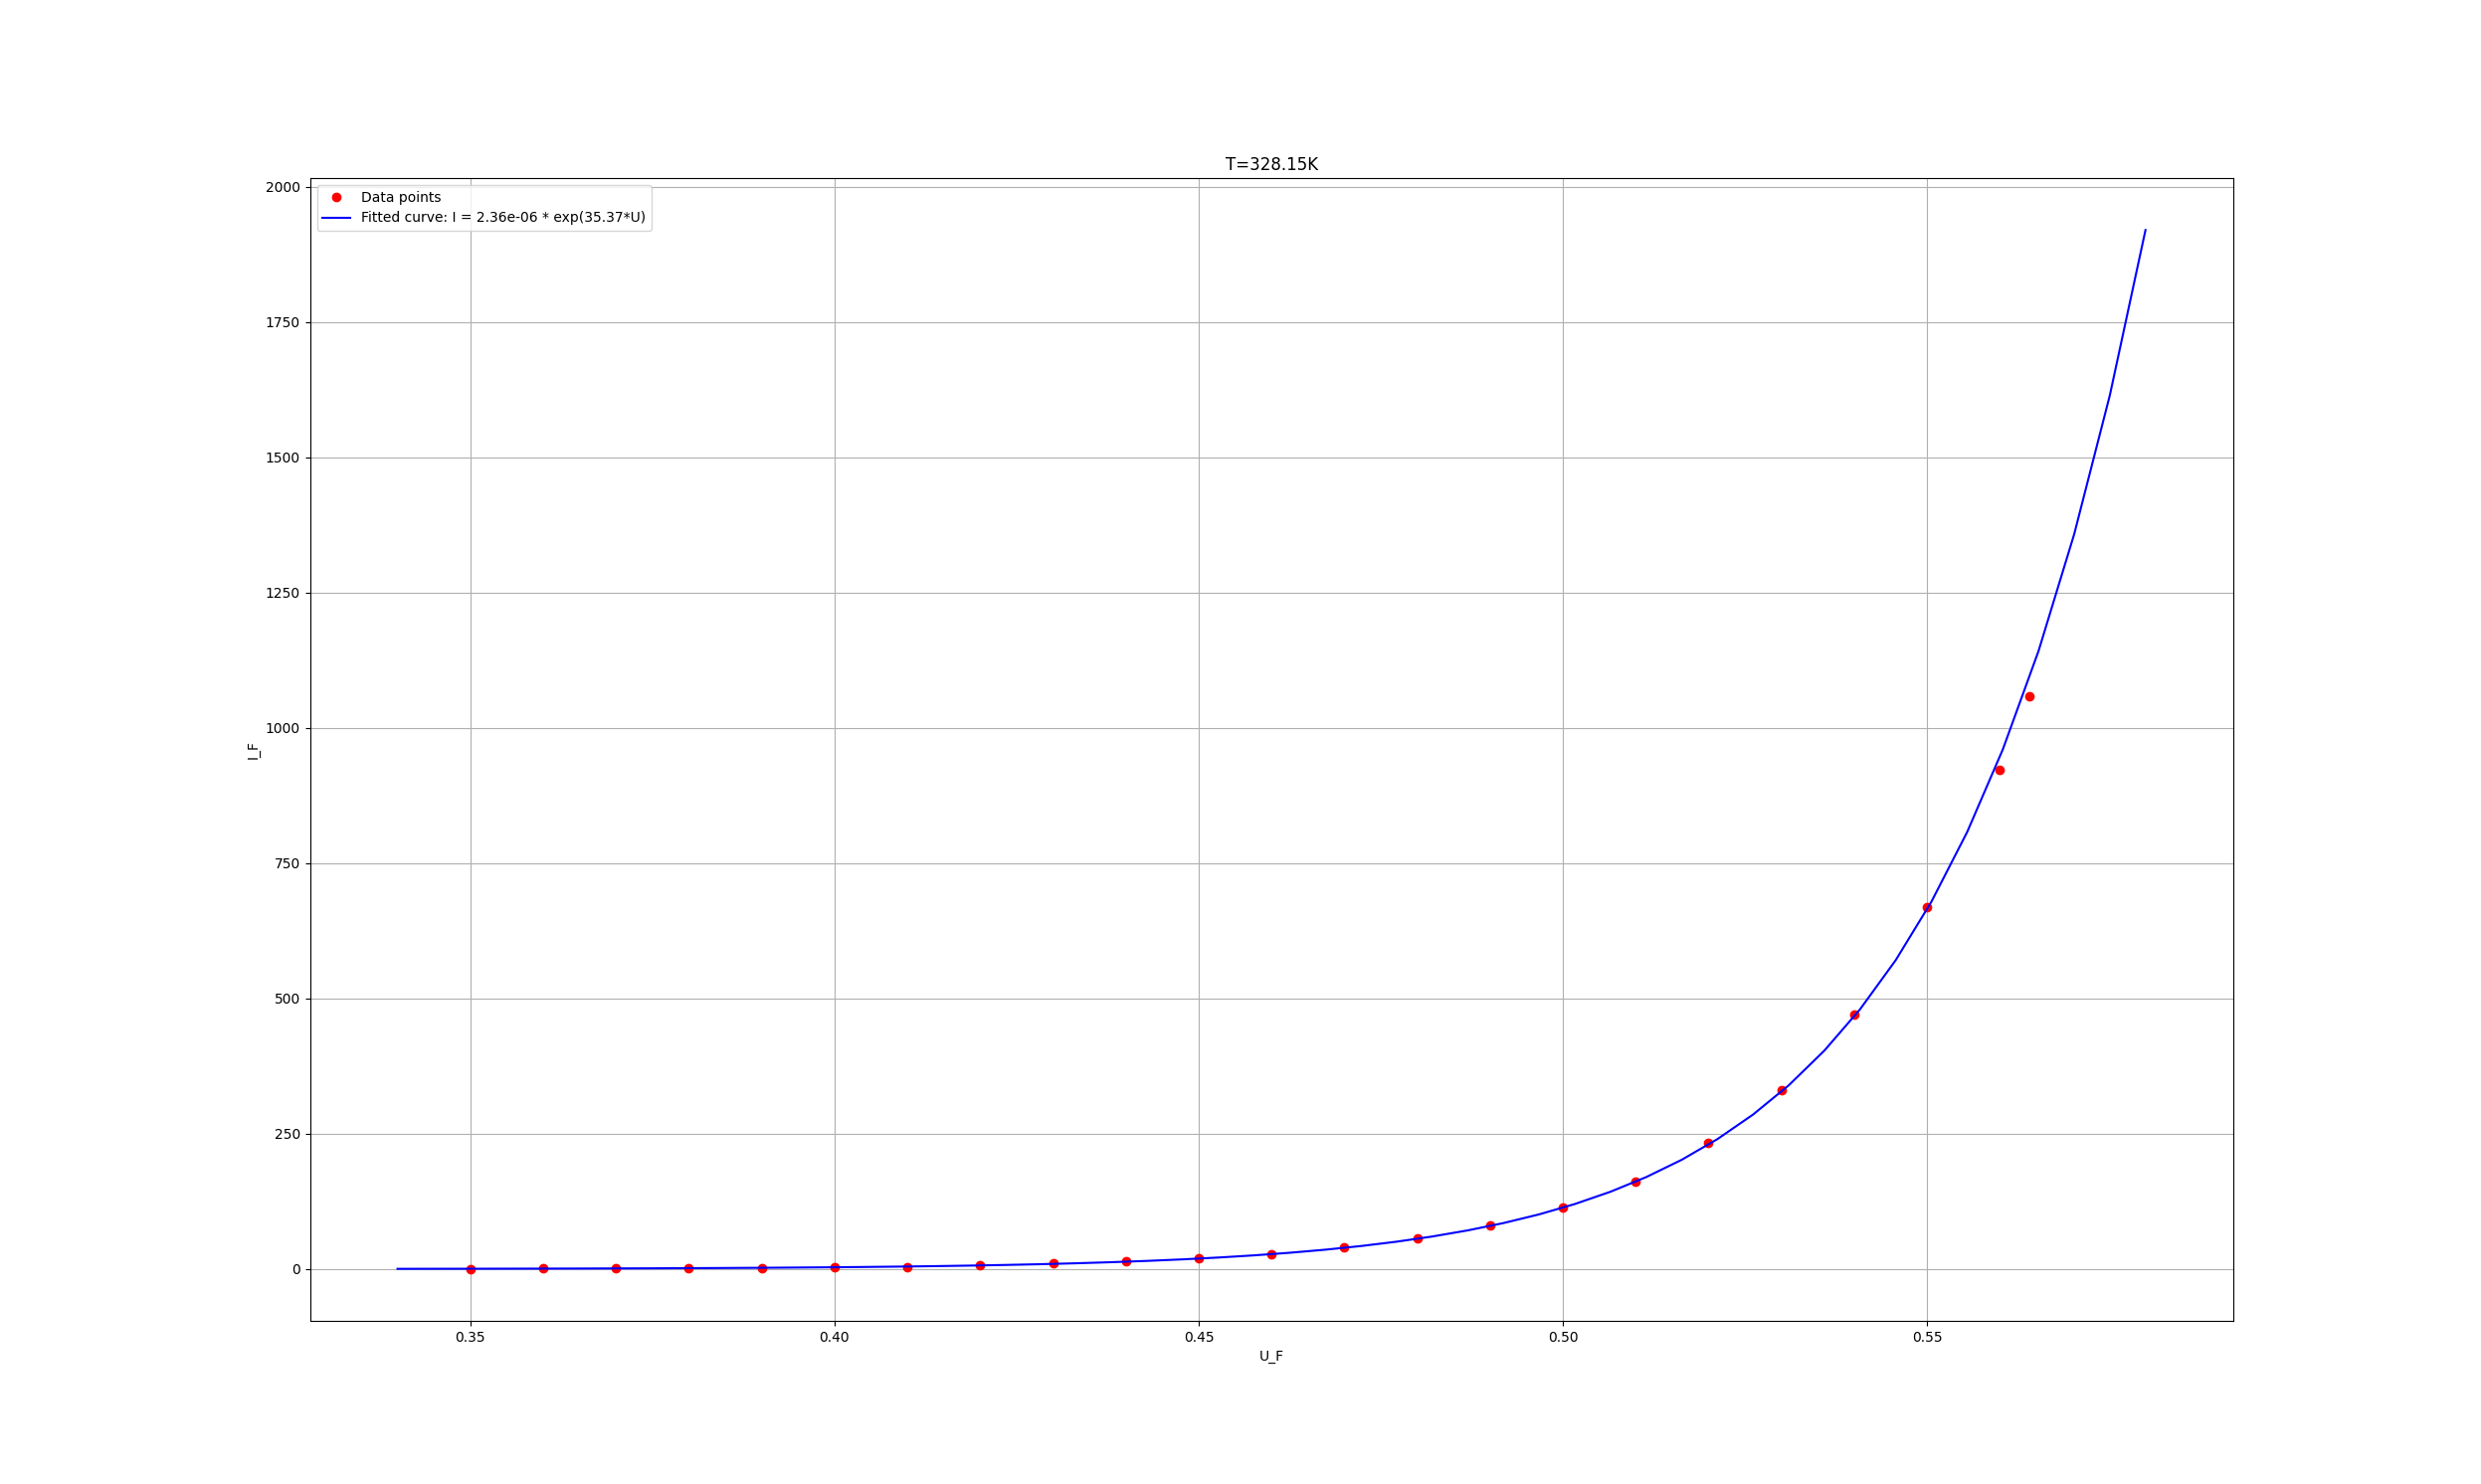
\includegraphics[width=\linewidth]{1.3.2.png}
			\caption{$I_F=2.36\times 10^{-6}e^{35.37U_F}$}
			\label{fig:sub6}
		\end{subfigure}
		\caption{$T=328.15K$}
		\label{fig3:combined}
	\end{figure}
	我们可以得到 \[I_s =2.36\times 10^{-6}\mu A,\frac{q}{kT} =35.37V^{-1}\]
	我们可以计算出 \[k = \frac{q}{T\times35.37V^{-1}} = \frac{1.6\times10^{-19}C}{328.15K\times35.37V^{-1}}=1.378518232\times10^{-23}J/K\]
	对于玻尔兹曼常数的公认值为\[k = 1.380649\times10^{-23} J/K\]
	我们的误差为\[\frac{|1.380649\times10^{-23} J/K-1.378518232\times10^{-23}J/K|}{1.380649\times10^{-23} J/K}\times100\%=0.15433\%\]
    }
    我们发现我们得到的三组玻尔兹曼常数和公认值的差距都非常小,相对误差控制在$1\%$以内,我们认为我们的实验结果非常好.\\
	\begin{figure}[H]
		\centering
		\begin{subfigure}{0.4\textwidth} % 第一个子图，宽度占文本的48%
			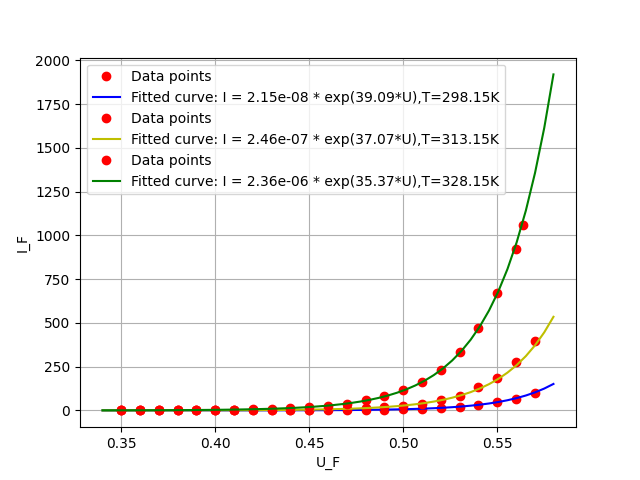
\includegraphics[width=\linewidth]{1.1.png}
			\caption{缩略版}
			\label{fig:sub7}
		\end{subfigure}
		\hfill % 填充水平间距
		\begin{subfigure}{0.4\textwidth} % 第二个子图
			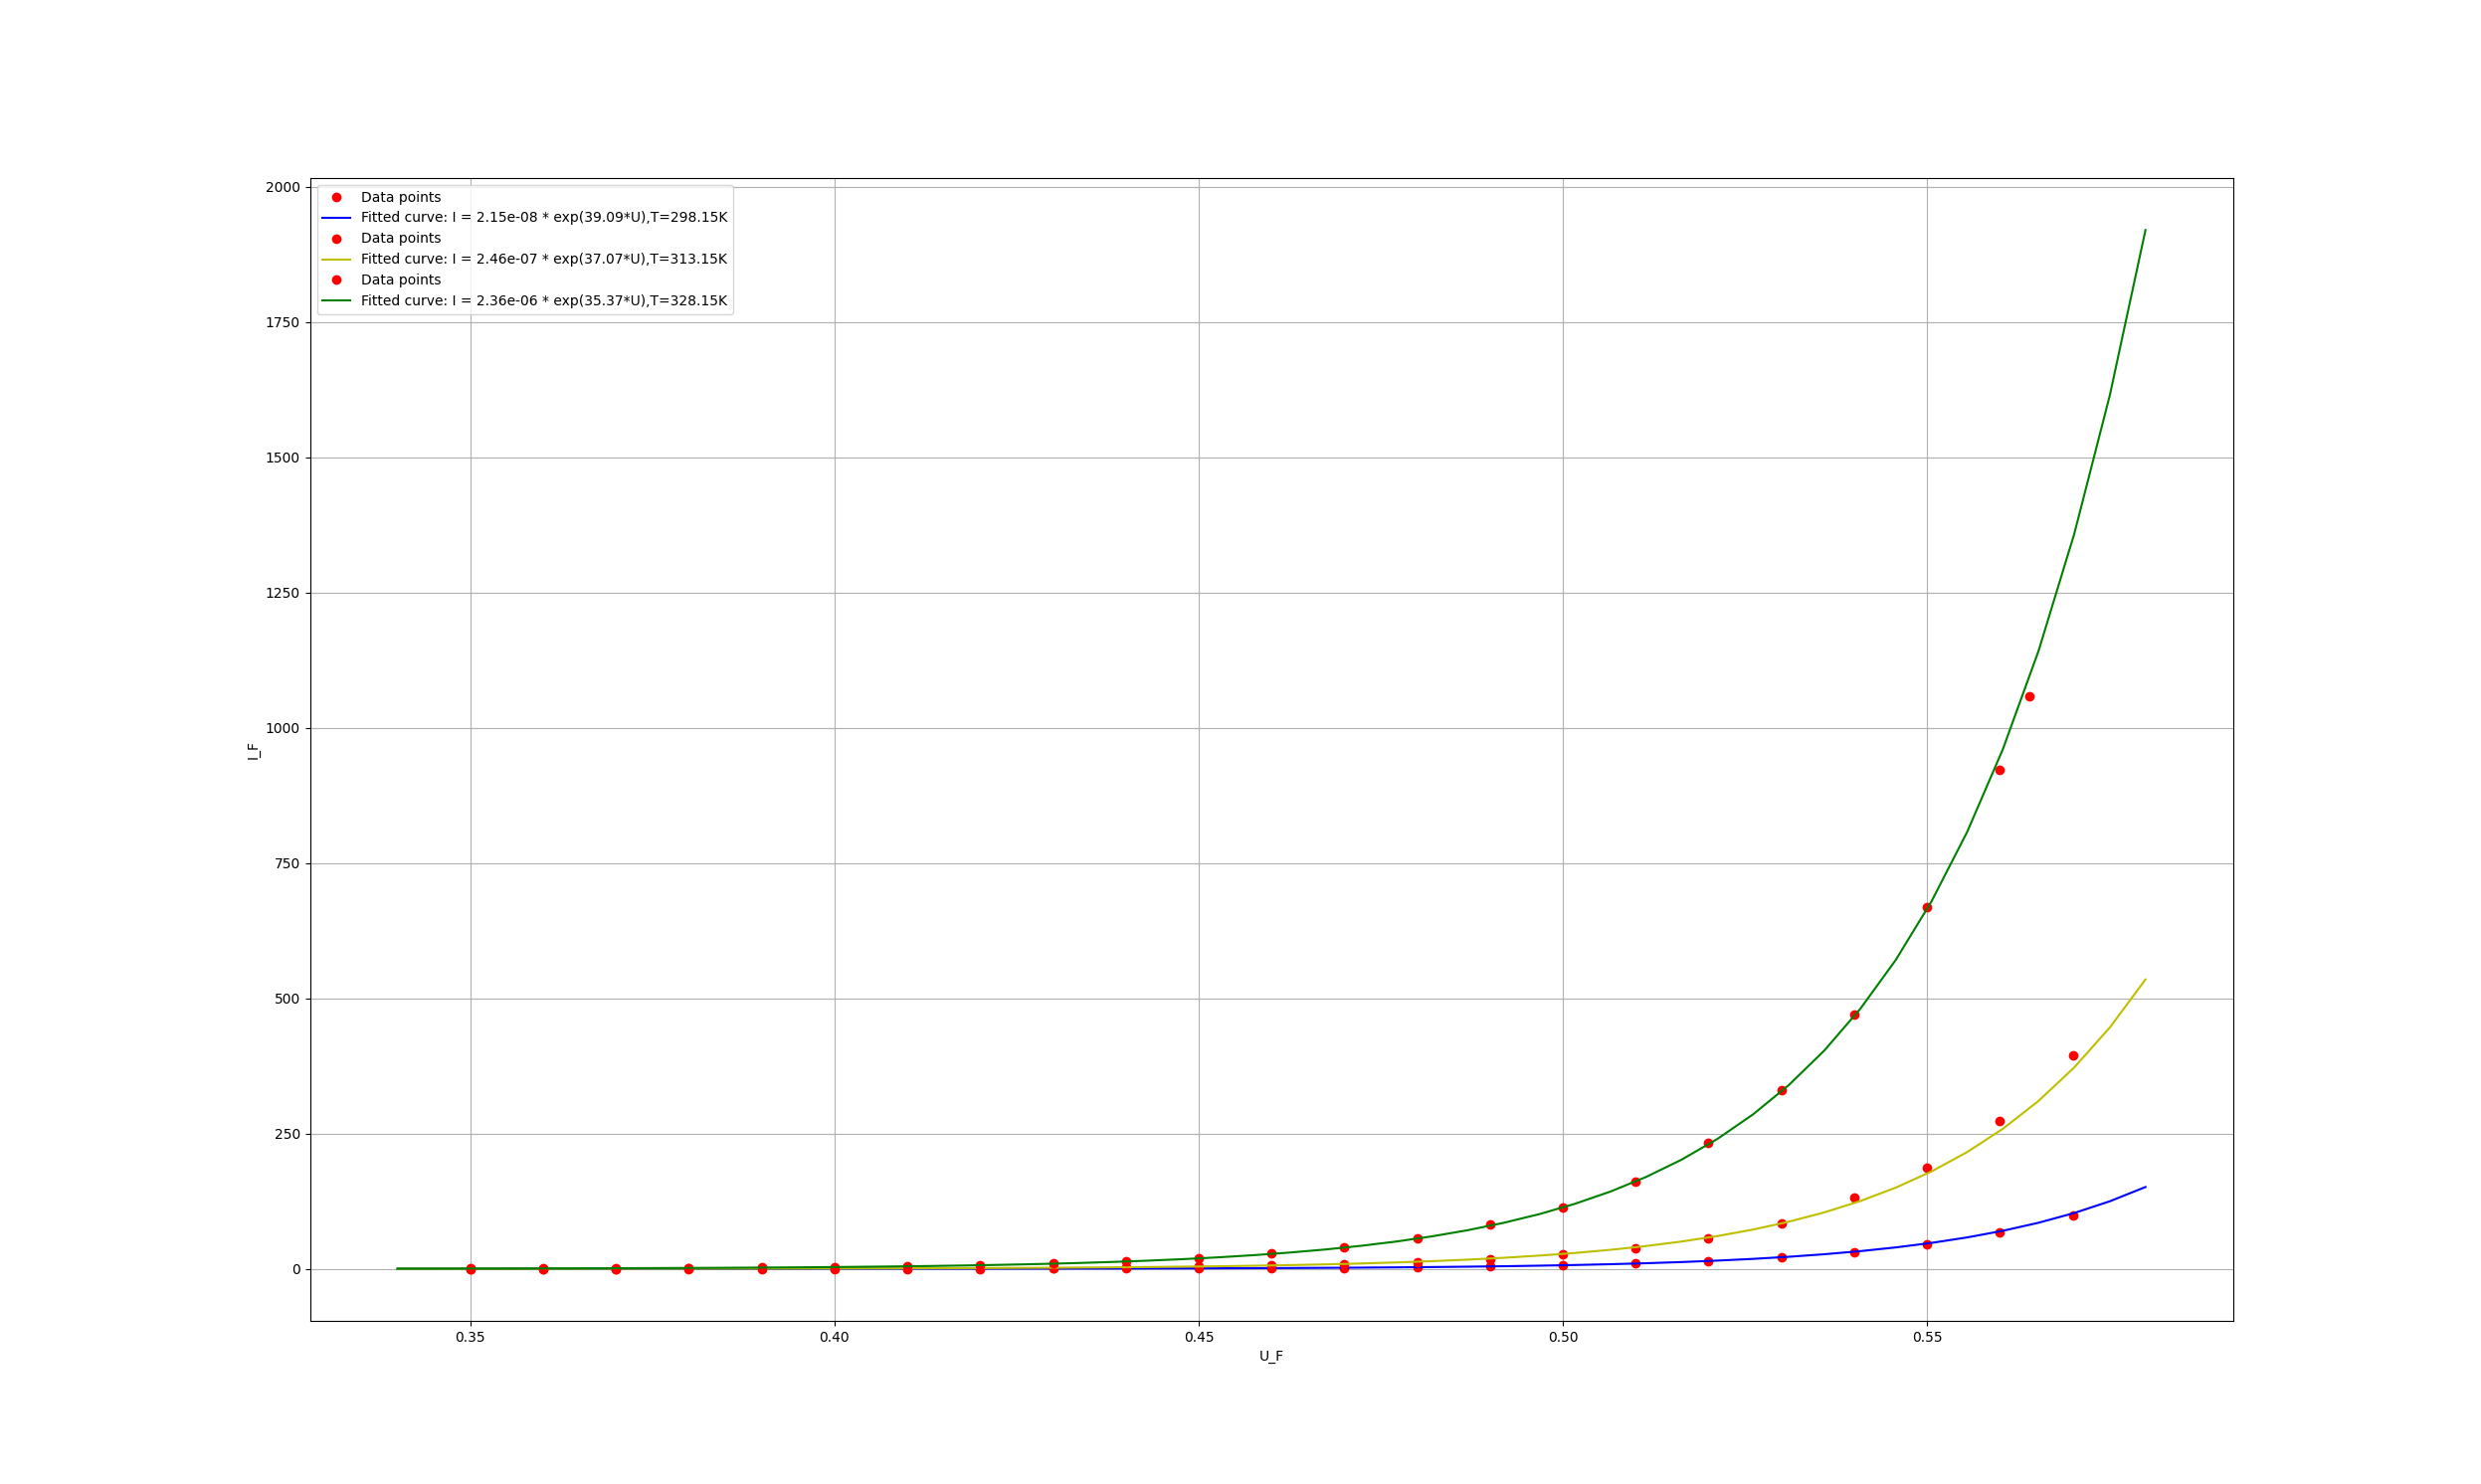
\includegraphics[width=\linewidth]{1.2.png}
			\caption{高清版}
			\label{fig:sub8}
		\end{subfigure}
		\caption{三条曲线}
		\label{fig4:combined}
	\end{figure}
	
	
	
	
	
	
	\section{升温曲线}
{
	\resizebox{\textwidth}{!}{ % 宽度撑满文本宽度，高度自动调整
			\begin{tabular}{|c|*{9}{c|}}
				\hline
				序号 &1 & 2 & 3 & 4 & 5 & 6 & 7 & 8 & 9 \\
				\hline
				$T^{o}C$ &28.100 & 30.000 & 40.000 & 50.000 & 60.000 & 70.000 & 80.000 & 90.000 & 100.000\\
				\hline
				$V_F$($V$) &0.546 & 0.540 & 0.519 & 0.487 & 0.463 & 0.438 & 0.413 & 0.388 & 0.364\\
				\hline
			\end{tabular}
}
	\begin{figure}[H]
		\centering
		\begin{subfigure}{0.48\textwidth} % 第一个子图，宽度占文本的48%
			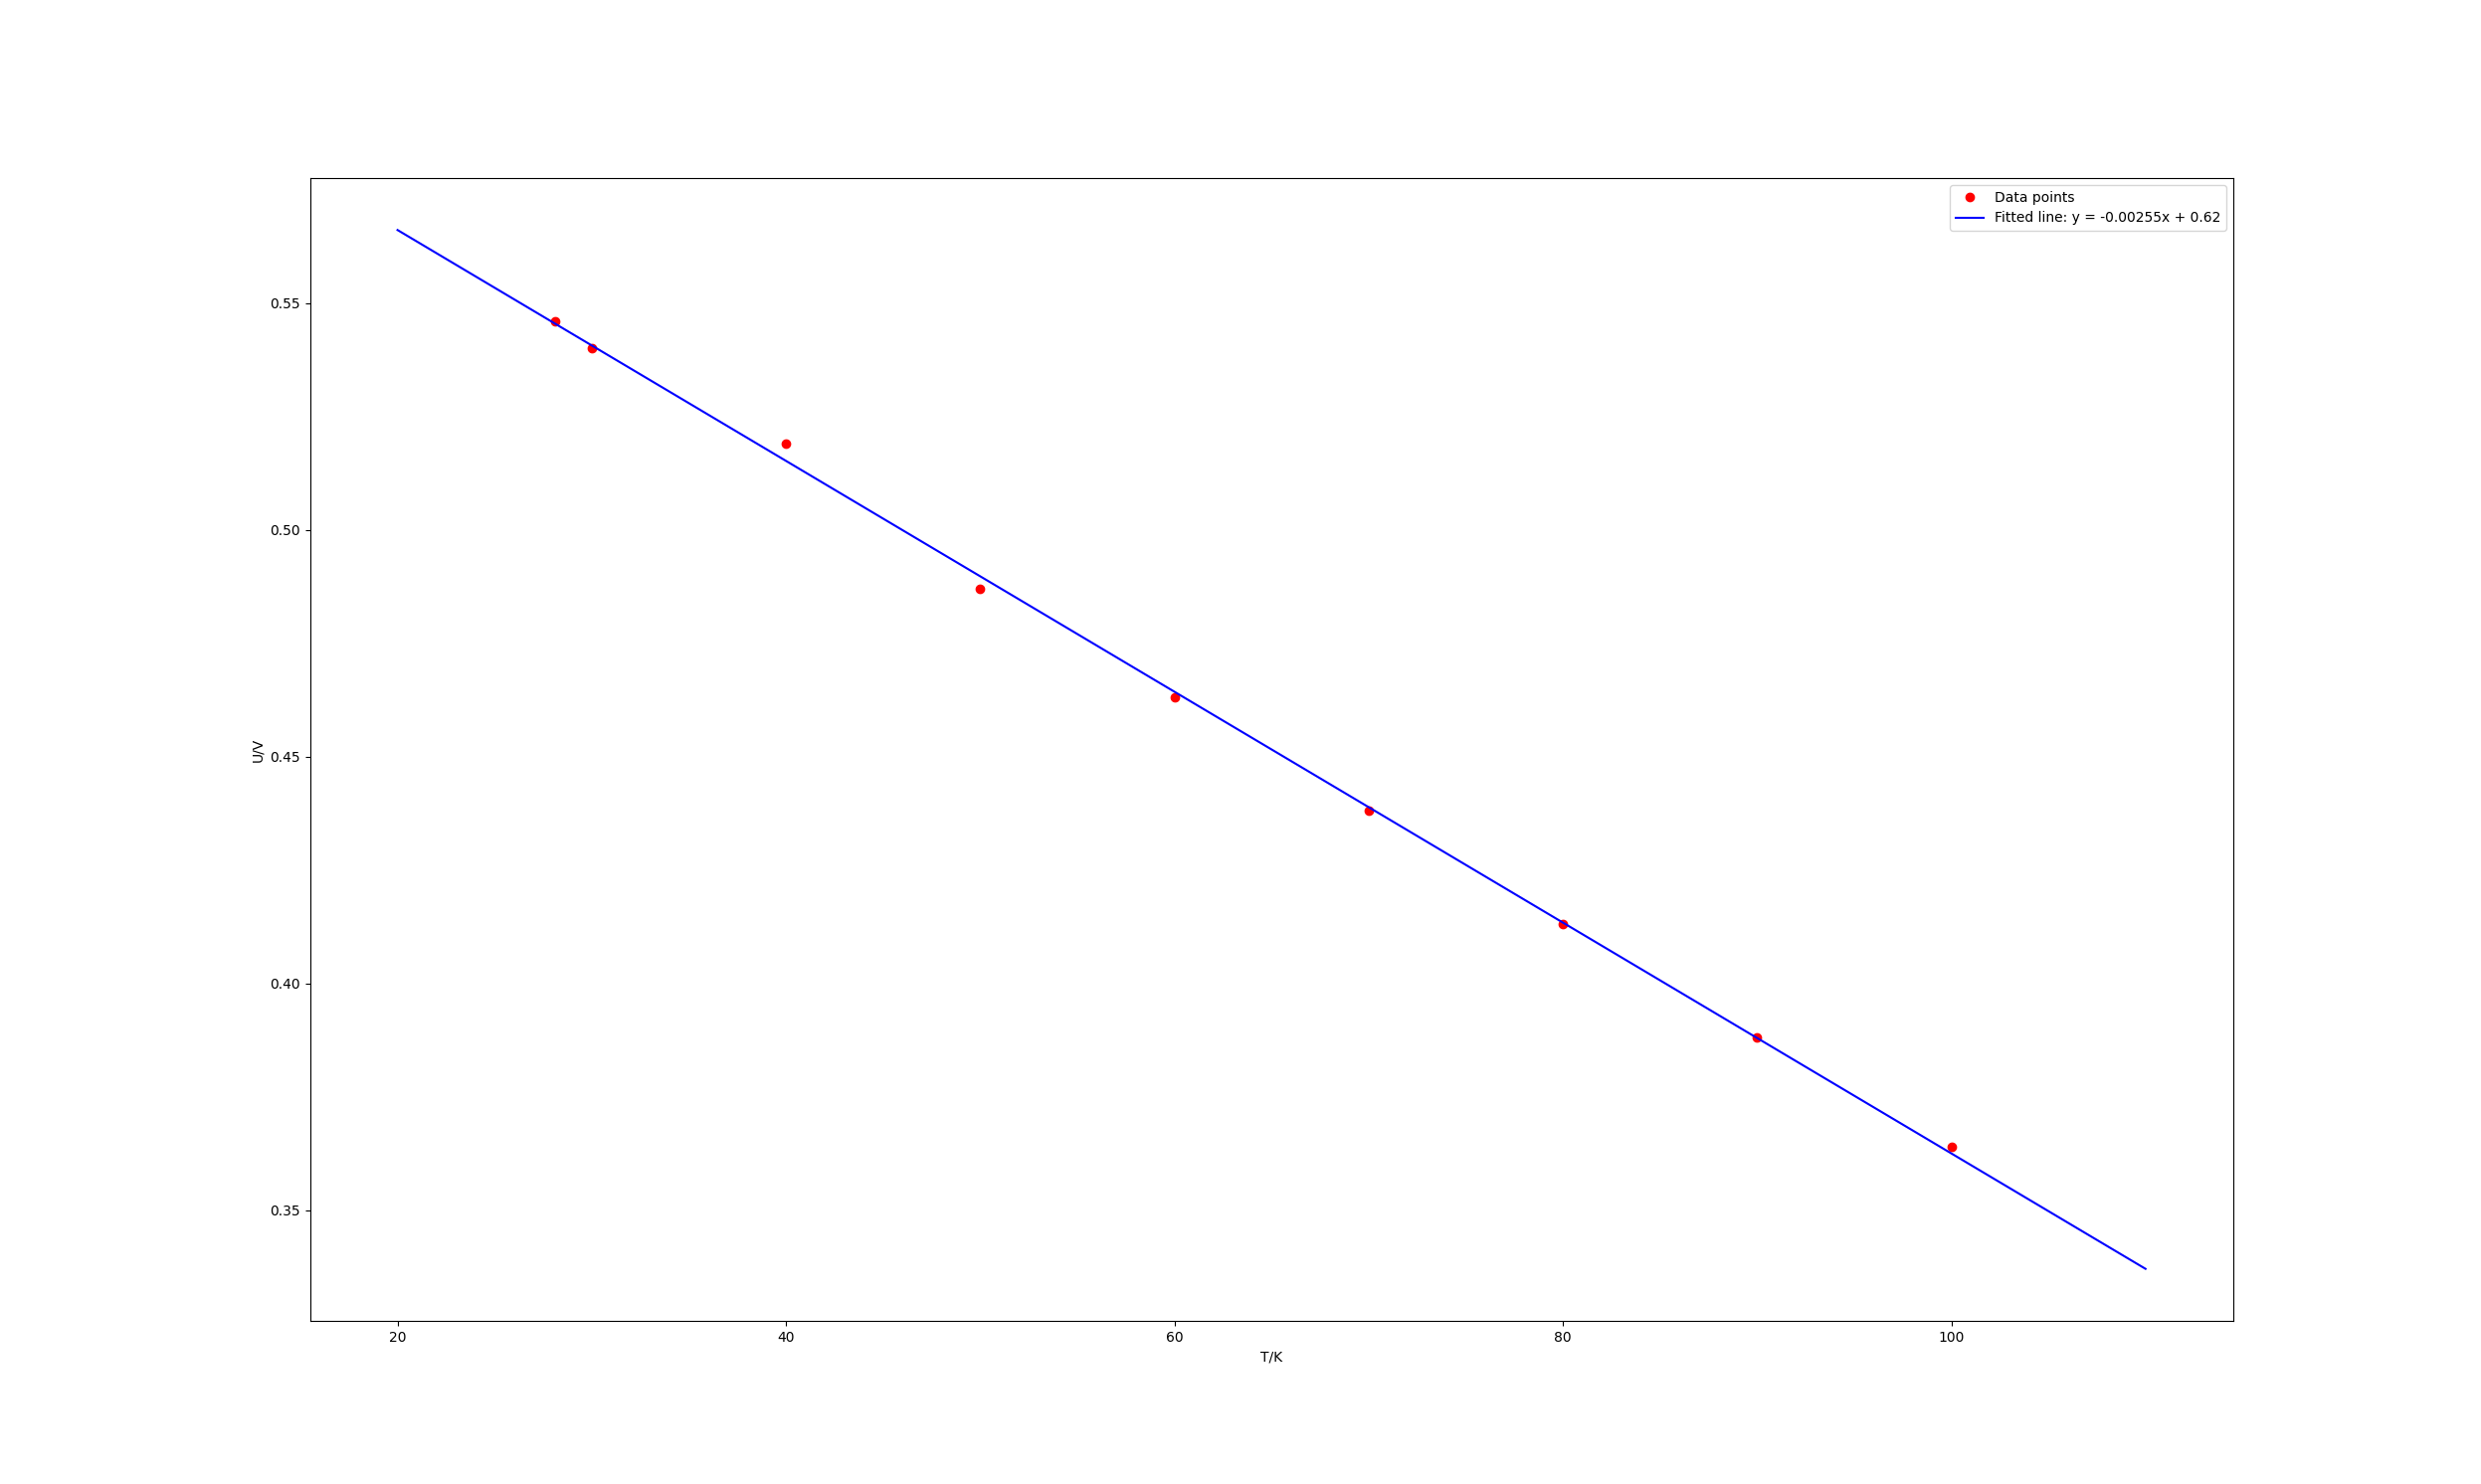
\includegraphics[width=\linewidth]{2.1.png}
			\caption{摄氏温标:$V_F=-0.00255T+0.62$}
			\label{fig:sub9}
		\end{subfigure}
		\hfill % 填充水平间距
		\begin{subfigure}{0.48\textwidth} % 第二个子图
			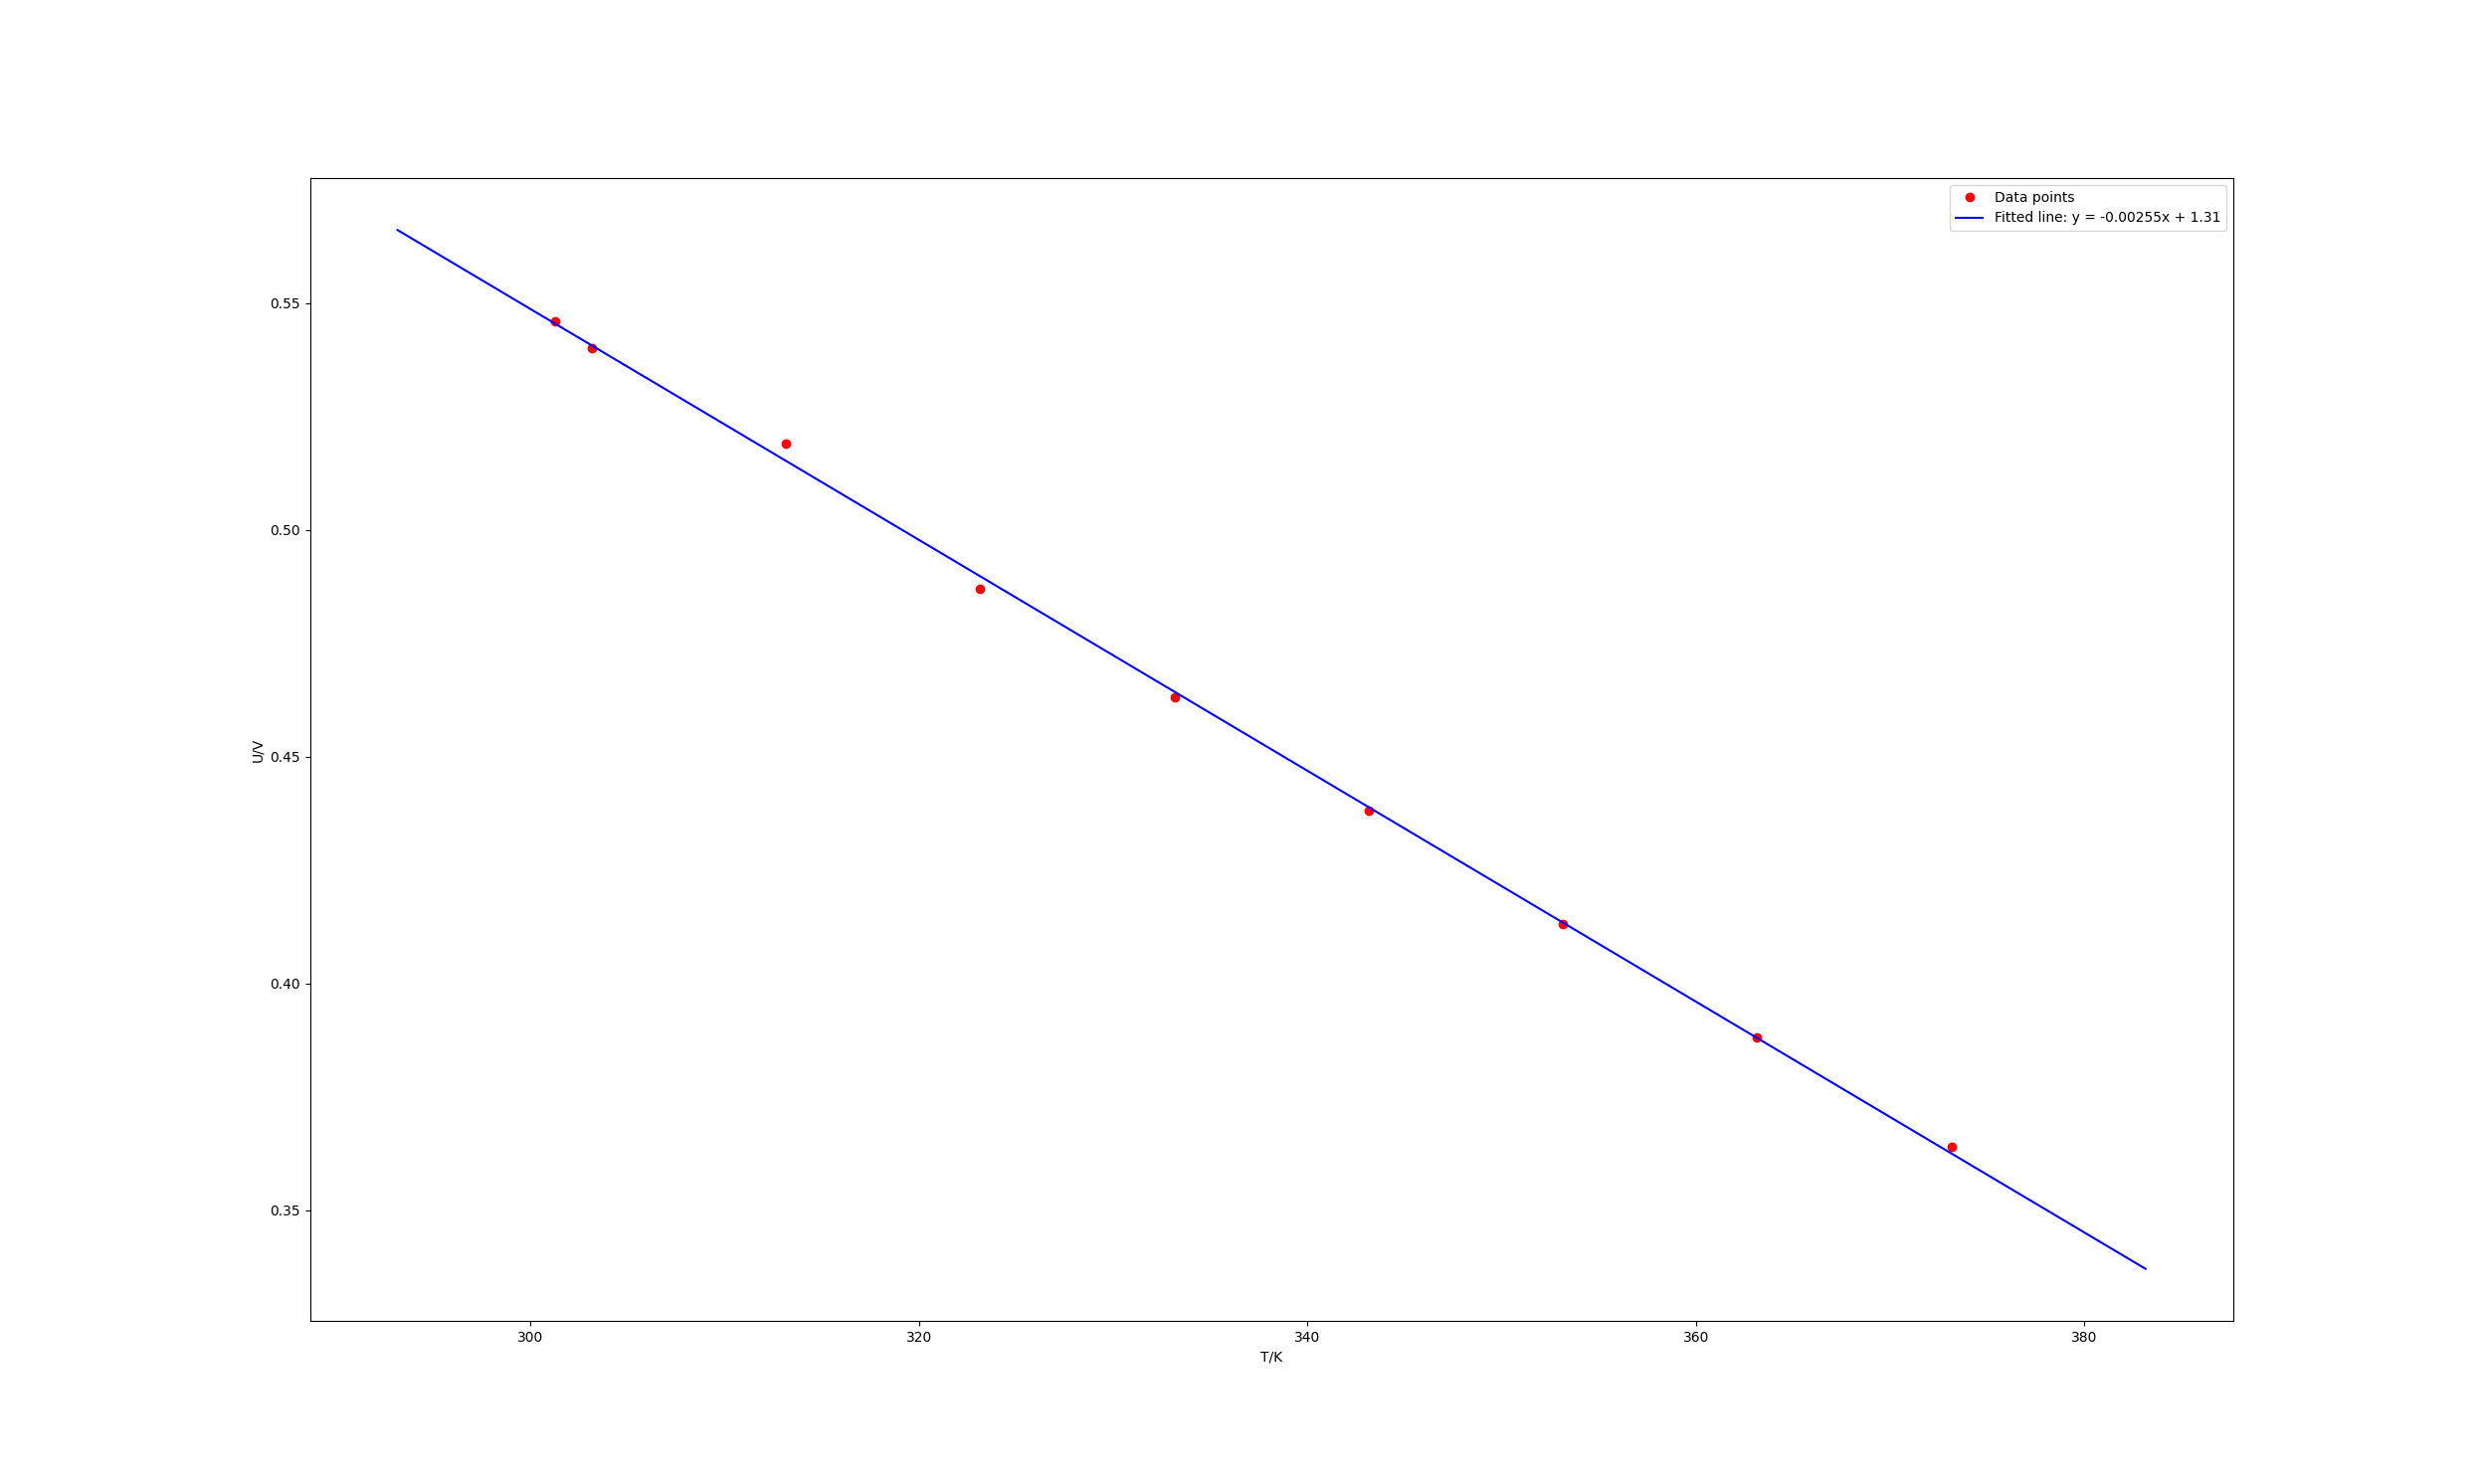
\includegraphics[width=\linewidth]{2.2.png}
			\caption{热力学温标:$V_F=-0.00255T+1.31$}
			\label{fig:sub10}
		\end{subfigure}
		\caption{三条曲线}
		\label{fig5combined}
	\end{figure}
	我们可以得到
	\[S = -\frac{k}{e}ln\frac{c}{I_F} = -0.00255V/K\]
	\[U_g = 1.31V\]
	\[E_g = U_g \times 1.6\times10^{-19} C= 2.096\times10^{-19}V\]
	对于$GaAs$类的半导体材料,其带隙为$1.43eV$,而我们的测值为$1.31eV$,相对误差为\[\frac{|1.43-1.31|}{1.31}=9.1603\%\]
\textbf{误差分析}:\\
温度控制不准确：禁带宽度$E_g$与温度$T$的关系为：
		\begin{equation*}
			E_g(T) = E_g(0) - \frac{\alpha T^2}{T+\beta}
			\quad (\text{Varshni方程})
		\end{equation*}
		若温控精度为$\pm \SI{1}{\celsius}$，可能导致$E_g$偏差约\SI{0.003}{\electronvolt}。

\end{document}